\section{Example problems} \label{sec:examples}

\subsection{Testing framework and the \class{TestProblem} class}
The \class{TestProblem} class is a framework for creating test problems. The code that implements the test problem itself is in the \texttt{solveProblem()} function of each class. The test problems described in the following section are summarized in table \ref{tbl:testproblems}. Each of these classes inherit from \class{TestProblem}.
\begin{table}[H]
	\begin{tabular}[c]{|l|p{5cm}|l|}
		\hline
		\textbf{Section} & \textbf{Problem} &  \textbf{Class name} \\
		\hline
		\ref{sec:farminglp} & Farming LP case & \class{FarmingLP} \\
		\hline
		\ref{sec:farmingqp} & Farming QP case & \class{FarmingQP} \\
		\hline
		\ref{sec:farminginteger} & Farming QP case with integer variables & \class{FarmingInteger} \\
		\hline
		\ref{sec:maxflow} & Network maximum flow case & \class{MaximumFlow} \\
		\hline		
		\ref{sec:maxflowrouting} & Network maximum flow with routing & \class{FlowWithRouting} \\
		\hline		
		\ref{sec:shcb_polynomial} & Six-Hump Camelback function: Local optimization with the \class{ConstraintPolynomial} constraint class & \class{SixHumpCamelPolynomial} \\
		\hline		
		\ref{sec:shcb_custom} & Six-Hump Camelback function: Local optimization with a custom constraint class & \class{SixHumpCamelCustom} \\
		\hline		
		\ref{sec:shcb_aBnB} & Six-Hump Camelback function: Global optimization using an alpha-Branch-and-Bound approach with custom constraint and relaxed constraint classes & \class{SixHumpCamelABnB} \\
		\hline		
		\ref{sec:shcb_bspline} & Six-Hump Camelback function: Global optimization using B-Spline approximation & \class{SixHumpCamelBSpline} \\
		\hline		
\end{tabular}
\caption{Test problems and their class names}
\label{tbl:testproblems}
\end{table}

\newpage
\subsection{Farming problem}
In this section we will look at a simple optimization problem taken from the lecture notes of the NTNU course TTK4135 Optimization and Control. We will look at three cases:
\begin{enumerate}
\item Linear programming case
\item Quadratic programming case
\item Introduction of integer variables
\end{enumerate}

\subsubsection{Linear programming case} \label{sec:farminglp}
We will start with a simple LP case. A farmer wants to grow apples and bananas. He has a field of size $100000\ \mathrm{m}^2$. Growing 1 tonne of apples requires an area of $4000\ \mathrm{m}^2$ and $60\ \mathrm{kg}$ of fertilizer. Growing 1 tonne of bananas requires an area of $3000\ \mathrm{m}^2$ and $80\ \mathrm{kg}$ of fertilizer. The profit for apples is 7000 per tonne (including fertilizer cost), and the profit for bananas is 6000 per tonne (including fertilizer cost). The farmer can legally use up to $2000\ \mathrm{kg}$ of fertilizer. He wants to maximize his profits.

\paragraph{Optimization variables.} We will introduce two optimization variables. $x_0$ is the number of tonnes of apples grown, and $x_1$ is the number of tonnes of bananas grown. We define a vector of optimization variables $x = [x_0, x_1]^\top$.

\paragraph{Objective function.} The farmer wants to maximize his profits, that is, he wants to
\[
\maximize 7000x_0 + 6000x_1.
\]
We want a minimization problem, so we negate the objective function and write it on standard LP form:
\[
\minimize \underbrace{\begin{bmatrix} -7000 & -6000 \end{bmatrix}}_{v^\top} \underbrace{\begin{bmatrix} x_0 \\ x_1 \end{bmatrix}}_x.
\]

\paragraph{Constraints.} In this problem, we have two constraints. The farmer cannot grow more than he has room for in the field:
\[
\underbrace{4000 x_0}_\mathrm{Area\ used\ for\ apples} + \underbrace{3000 x_1}_\mathrm{Area\ used\ for\ bananas} \leq \underbrace{100000}_\mathrm{Available\ area}.
\]
He cannot exceed the legal amount of fertilizer used:
\[
\underbrace{60 x_0}_\mathrm{Fertilizer\ used\ for\ apples} + \underbrace{80 x_1}_\mathrm{Fertilizer\ used\ for\ bananas} \leq \underbrace{2000}_\mathrm{Legal\ amount\ of\ fertilizer}.
\]
We want a constraint on the form $Ax \leq b$, so we write
\[
\underbrace{\begin{bmatrix} 4000 & 3000 \\ 60 & 80 \end{bmatrix}}_A \underbrace{\begin{bmatrix} x_0 \\ x_1 \end{bmatrix}}_x \leq \underbrace{\begin{bmatrix} 100000 \\ 2000 \end{bmatrix}}_b
\]

\paragraph{Variable bounds.}
We also have nonnegativity constraints on the optimization variables (he cannot grow negative amounts). These are included in the variable bounds:
\[
0 \leq x \leq \infty.
\]

\paragraph{Optimization problem.} We now have the optimization problem
\begin{subequations}
\begin{align}
\minimize v^\top x \\
\subto Ax &\leq b \\
0 \leq x &\leq \infty
\end{align}
\end{subequations}
The problem is illustrated in fig. \ref{fig:farmingLP}.

\begin{figure}[H]
\centering
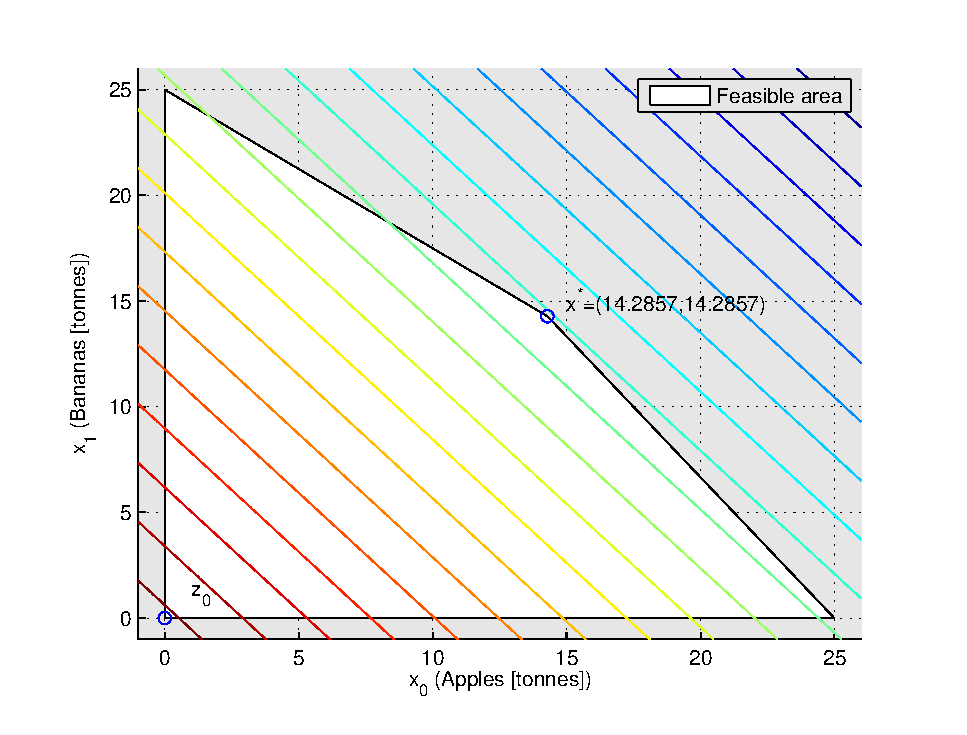
\includegraphics[width=\textwidth]{figures/FarmingLP.eps}
\caption{Graphical representation of the farming LP. The optimal point at $x^*=(14.2857,14.2857)$ and starting point $z_0 = (0,0)$ are marked with blue circles.}
\label{fig:farmingLP}
\end{figure}

\paragraph{Setting up and solving the problem.}
We set up a new \class{TestProblem} class called \class{FarmingLP}. The code below is implemented in the \texttt{solveProblem()} function to set up and solve the farming LP.
\begin{lstlisting}[numbers=left]
void FarmingLP::solveProblem()
{
	// Variable bounds
    std::vector< double > lb {0, 0};
    std::vector< double > ub {INF, INF};
    // Starting point
    std::vector< double > z0 {0, 0};
    // Objective function
    DenseMatrix v(1, 2);
    v << -7000, -6000;
    ObjectivePtr objective(new ObjectiveLinear(v));
    // Constraints
    DenseMatrix A(2, 2);
    A << 4000,  3000,
           60,    80;
    DenseVector b(2);
    b << 100000,
           2000;
    ConstraintPtr cLinear(new ConstraintLinear(A, b, false));
    // Constraint composite
    ConstraintCompositePtr constraints(new ConstraintComposite(2, lb, ub));
    constraints->add(cLinear);
    // Optimize
    OptimizerIpopt optIpopt(objective, constraints, z0);
    int status = optIpopt.optimize();
    fopt_found = optIpopt.getObjectiveValue();
    zopt_found = optIpopt.getOptimalSolution();
    cout << "Optimal solution: f*=" << fopt_found << endl;
    cout << "Optimal point: x*=(" << zopt_found.at(0) << "," << zopt_found.at(1) << ")" << endl;
}
\end{lstlisting}
Lines 4-7 declare and fill STL vectors with the lower variable bounds, upper variable bounds and starting point. Lines 8-11 define the objective function. Lines 12-19 define the linear constraints. Lines 20-22 create a constraint composite and inserts the linear constraint. Lines 23-25 creates an Ipopt optimizer object and solves the problem. Lines 26-29 extracts and prints information about the solution. When used in the \class{TestProblem} framework, this gives us the printout
\newline
{\footnotesize{\texttt{Running Farming LP problem...\\
\\
******************************************************************************\\
This program contains Ipopt, a library for large-scale nonlinear optimization.\\
 Ipopt is released as open source code under the Eclipse Public License (EPL).\\
         For more information visit http://projects.coin-or.org/Ipopt\\
******************************************************************************\\
\\
Optimal solution: f*=-185714\\
Optimal point: x*=(14.2857,14.2857)\\
Farming LP problem successfully solved in 0 (ms)\\
Press <RETURN> to close this window...\\
}}}
We see that the correct optimal solution is found, as expected. The maximum profit is 185714.

\subsubsection{Quadratic programming case} \label{sec:farmingqp}
Now consider a case where the price of apples and bananas depends on how much is produced. Now the profit for apples is $7000-200x_0$ per tonne (including fertilizer cost) and the profit for bananas is $4000-140x_1$ per tonne (including fertilizer cost). All the other parameters of the problem (field size, fertilizer limit etc.) are the same as for the LP case. We want a linear objective function, so we introduce a new variable $x_2$ to represent the profit:
\begin{align*}
x_2 &= (7000-200x_0)x_0 + (4000-140x_1)x_1 \\
&= \begin{bmatrix} x_0 & x_1 \end{bmatrix} \begin{bmatrix} -200 & 0 \\ 0 & -140 \end{bmatrix} \begin{bmatrix} x_0 \\ x_1 \end{bmatrix} + \begin{bmatrix} 7000 & 4000 \end{bmatrix} \begin{bmatrix} x_0 \\ x_1 \end{bmatrix}.
\end{align*}

\paragraph{Optimization variables.}
We redefine our vector of optimization variables to be $x = [x_0, x_1, x_2]^\top$. Here, $x_0$ and $x_1$ represent the same as before, and the new variable $x_2$ is the profit.

\paragraph{Objective function.} Since $x_2$ represents profit and we want to maximize this, our new objective is
\[
\minimize \underbrace{\begin{bmatrix} 0 & 0 & -1 \end{bmatrix}}_{v^\top} \underbrace{\begin{bmatrix} x_0 \\ x_1 \\ x_2 \end{bmatrix}}_x.
\]

\paragraph{Constraints.} We keep the linear constraint from the LP case:
\[
A \begin{bmatrix} x_0 \\ x_1 \end{bmatrix} \leq b.
\]
We also have to create a constraint to define the relationship between the three variables. We have
\[
x_2 - \left( \begin{bmatrix} x_0 & x_1 \end{bmatrix} \begin{bmatrix} -200 & 0 \\ 0 & -140 \end{bmatrix} \begin{bmatrix} x_0 \\ x_1 \end{bmatrix} + \begin{bmatrix} 7000 & 4000 \end{bmatrix} \begin{bmatrix} x_0 \\ x_1 \end{bmatrix} \right) = 0,
\]
which we can write as
\[
0 \leq x^\top \underbrace{\begin{bmatrix} 200 & 0 & 0 \\ 0 & 140 & 0 \\ 0 & 0 & 0 \end{bmatrix}}_P x+ \underbrace{\begin{bmatrix} -7000 & -4000 & 1 \end{bmatrix}}_{q^\top} x \leq 0,
\]
that is, we can use the \class{ConstraintQuadratic} class to define this constraint.

\paragraph{Variable bounds.} Both $x_0$ and $x_1$ have to be nonnegative as before, but $x_2$ can in principle also be negative (meaning the farmer is losing money). Therefore, the bounds are
\begin{align*}
0 &\leq x_0 \leq \infty \\
0 &\leq x_1 \leq \infty \\
-\infty &\leq x_2 \leq \infty \\
\end{align*}

\paragraph{Optimization problem.} We now have the optimization problem
\begin{subequations}
\begin{align}
\minimize v^\top x \\
\subto A \begin{bmatrix} x_0 \\ x_1 \end{bmatrix} &\leq b, \\
0 \leq x^\top P x + q^\top x &\leq 0, \\
0 \leq \begin{bmatrix} x_0 \\ x_1 \end{bmatrix} &\leq \infty, \\
-\infty \leq x_2 &\leq \infty.
\end{align}
\end{subequations}
The problem is illustrated in fig. \ref{fig:farmingQP}.

\begin{figure}[H]
\centering
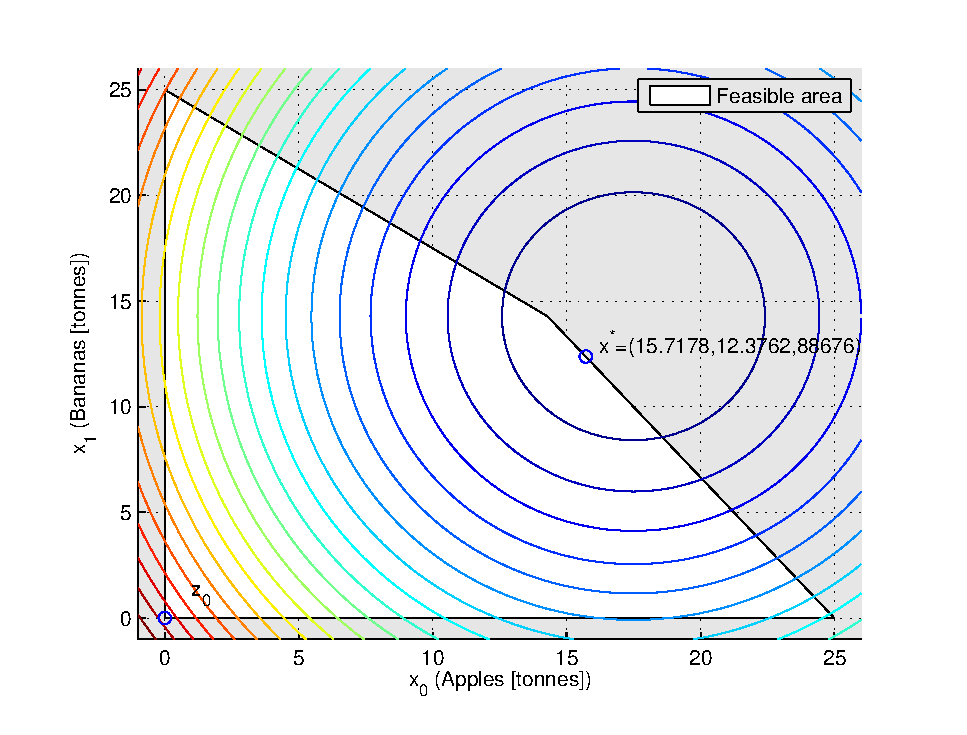
\includegraphics[width=\textwidth]{figures/FarmingQP.eps}
\caption{Graphical representation of the farming QP. The optimal point at $x^*=(15.7178,12.3762,88676)$ and starting point $z_0 = (0,0,0)$ are marked with blue circles.}
\label{fig:farmingQP}
\end{figure}

\paragraph{Setting up and solving the problem.}
We set up a new \class{TestProblem} class called \class{FarmingQP}. The code below is implemented in the \texttt{solveProblem()} function to set up and solve the farming QP.
\begin{lstlisting}[numbers=left]
void FarmingQP::solveProblem()
{
	// Variable bounds
    std::vector< double > lb {0, 0, -INF};
    std::vector< double > ub {INF, INF, INF};
    // Starting point
    std::vector< double > z0 {0, 0, 0};
    // Objective function
    DenseMatrix v(1, 3);
    v << 0, 0, -1;
    ObjectivePtr objective(new ObjectiveLinear(v));
    // Linear constraint
    DenseMatrix A(2, 2);
    A << 4000,  3000,
           60,    80;
    DenseVector b(2);
    b << 100000,
           2000;
    ConstraintPtr cLinear(new ConstraintLinear(A, b, false));
    // Linear constraint variable mapping
    std::vector< int > varMapLinear {0, 1};
    // Quadratic constraint
    DenseMatrix P(3, 3);
    P << 200,   0, 0,
           0, 140, 0,
           0,   0, 0;
    DenseMatrix q(3, 1);
    q << -7000,
         -4000,
             1;
    ConstraintPtr cQuadratic(new ConstraintQuadratic(P, q, 0, 0, 0));
    // Constraint composite
    ConstraintCompositePtr constraints(new ConstraintComposite(3, lb, ub));
    constraints->add(cLinear, varMapLinear);
    constraints->add(cQuadratic);
    // Optimize
    OptimizerIpopt optIpopt(objective, constraints, z0);
    int status = optIpopt.optimize();
    fopt_found = optIpopt.getObjectiveValue();
    zopt_found = optIpopt.getOptimalSolution();
    cout << "Optimal solution: f*=" << fopt_found << endl;
    cout << "Optimal point: x*=(" << zopt_found.at(0) << "," << zopt_found.at(1) << "," << zopt_found.at(2) << ")" << endl;
}
\end{lstlisting}
Lines 3-7 declare and fill STL vectors with the lower variable bounds, upper variable bounds and starting point. Lines 8-11 define the objective function. Lines 12-19 define the linear constraint. Line 21 defines an STL vector of integers which defines the mapping between the variables in the linear constraint (which has two variables) and the variables in the constraint composite (which has three variables). Lines 22-31 define the quadratic constraint. Lines 32-25 create a constraint composite and inserts the linear and quadratic constraints. Lines 36-38 creates an Ipopt optimizer object and solves the problem. Lines 39-42 extracts and prints information about the solution. When used in the \class{TestProblem} framework, this gives us the printout
\newline
{\footnotesize{\texttt{Running Farming QP problem...\\
\\
******************************************************************************\\
This program contains Ipopt, a library for large-scale nonlinear optimization.\\
 Ipopt is released as open source code under the Eclipse Public License (EPL).\\
         For more information visit http://projects.coin-or.org/Ipopt\\
******************************************************************************\\
\\
Optimal solution: f*=-88675.7\\
Optimal point: x*=(15.7178,12.3762,88675.7)\\
Farming QP problem successfully solved in 10 (ms)\\
Press <RETURN> to close this window...\\
}}}
We see that the correct optimal solution is found, as expected. The maximum profit is 88675.7.

\subsubsection{Integer variables} \label{sec:farminginteger}
We now say that the farmer is only allowed to produce integer amounts of apples and bananas. That is, we impose the additional constraint that $x_0$ and $x_1$ are integers. Since the objective function is linear, and the original constraints are convex, this becomes a convex MINLP. This is easily formulated and solved in a Branch-and-Bound framework.

\begin{figure}[H]
\centering
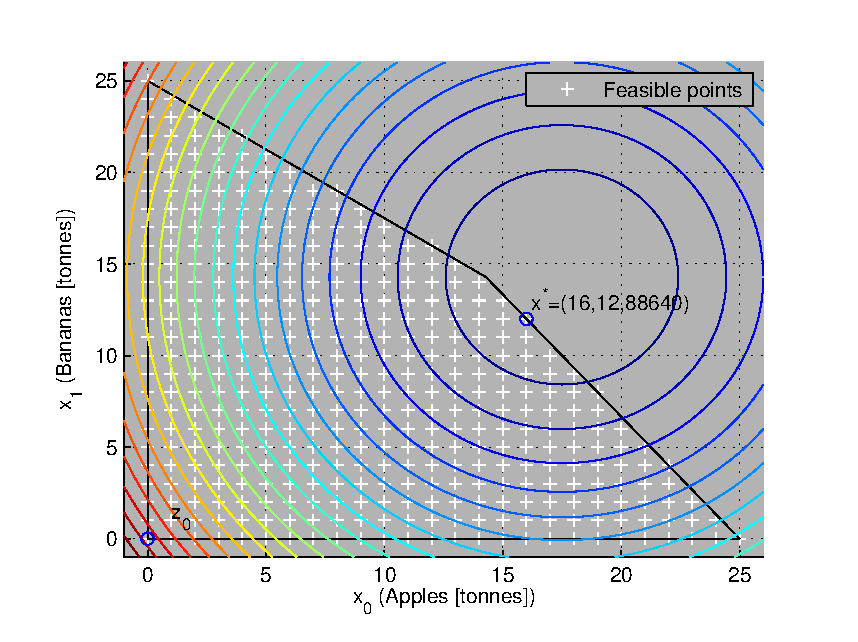
\includegraphics[width=\textwidth]{figures/FarmingInteger.eps}
\caption{Graphical representation of the farming problem with integer variables. The optimal point at $x^*=(16,12,88640)$ and starting point $z_0 = (0,0,0)$ are marked with blue circles.}
\label{fig:farmingInteger}
\end{figure}

\paragraph{Setting up and solving the problem.} We set up a new \class{TestProblem} class called \class{FarmingInteger}. The code below is implemented in the \texttt{solveProblem()} function to set up and solve the farming problem with integer variables.
\begin{lstlisting}[numbers=left]
void FarmingInteger::solveProblem()
{
	// Variable bounds
    std::vector< double > lb {0, 0, -INF};
    std::vector< double > ub {30, 30, INF};
    // Starting point
    std::vector< double > z0 {0, 0, 0};
    // Objective function
    DenseMatrix v(1, 3);
    v << 0, 0, -1;
    ObjectivePtr objective(new ObjectiveLinear(v));
    // Linear constraint
    DenseMatrix A(2, 2);
    A << 4000,  3000,
           60,    80;
    DenseVector b(2);
    b << 100000,
           2000;
    ConstraintPtr cLinear(new ConstraintLinear(A, b, false));
    // Linear constraint variable mapping
    std::vector< int > varMapLinear;
    varMapLinear.push_back(0);
    varMapLinear.push_back(1);
    // Quadratic constraint
    DenseMatrix P(3, 3);
    P << 200,   0, 0,
           0, 140, 0,
           0,   0, 0;
    DenseMatrix q(3, 1);
    q << -7000,
         -4000,
             1;
    ConstraintPtr cQuadratic(new ConstraintQuadratic(P, q, 0, 0, 0));
    // Constraint composite
    ConstraintCompositePtr constraints(new ConstraintComposite(3, lb, ub));
    constraints->add(cLinear, varMapLinear);
    constraints->add(cQuadratic);
	// Variable types
    std::vector< int > variable_types;
    variable_types.push_back(INTEGER); // x0
    variable_types.push_back(INTEGER); // x1
    variable_types.push_back(CONTINUOUS); // x2
	// Branching variables
    std::vector< int > branching_variables;
    branching_variables.push_back(0); // x0
    branching_variables.push_back(1); // x1
    // Optimize
    BranchAndBound bnb(objective, constraints, z0, variable_types, branching_variables);
    int status = bnb.optimize();
    fopt_found = bnb.getObjectiveValue();
    zopt_found = bnb.getOptimalSolution();
}
\end{lstlisting}
This is very similar to the QP case. The differences are:
\begin{itemize}
\item
In line 5, the upper bounds of $x_0$ and $x_1$ are set to 30 instead of $\infty$. This is because we are branching on these variables, so we must define an upper bound so that the Branch-and-Bound algorithm is able to calculate where to split the variable when branching. 30 is a reasonable choice as an upper bound, because there is not room to grow 30 tons of either fruit.
\item
Lines 38-42 define the variable types. Here, we have defined that $x_0$ and $x_1$ are integer variables, and $x_2$ (the profit function) is continuous.
\item
Lines 43-46 define which variables are to be branched on. Typically, we choose our degrees of freedom as branching variables; in our case, the amount of apples $x_0$ and the amount of bananas $x_1$.
\item
In lines 47-49, we use the \class{BranchAndBound} class instead of the \class{OptimizerIpopt} class. This is because we have integer variables and need to use branching to solve the problem.
\end{itemize}
When used in the \class{TestProblem} framework, this gives us the following output:
\newline
{\footnotesize{\texttt{Branch and Bound tree search finished after 19 iterations, using 0 sec.\\
Global solution upper bound = -88640\\
Global solution lower bound = -88640\\
Optimality gap = 0 <= 0.001 (epsilon)\\
Optimal point x* = (    16,     12, 8.864e+04)\\
\\
Farming QP problem successfully solved in 180 (ms)\\
Press <RETURN> to close this window...\\
}}}
We see that the correct optimal solution is found (quickly). The maximum profit is 88640.

\newpage
\subsection{Network flow problem}
Now we will look at some cases of network flow. Throughout this section we will look at a simple flow network with one source vertex, one sink vertex, four internal vertices and ten edges. The flow network is illustrated in fig. \ref{fig:flownetwork}. We denote the vertices $v_i,\ i = \lbrace 0 \dots 5 \rbrace$ and the edges $e_j,\ j = \lbrace 0 \dots 9 \rbrace$. For context, we could say the flow network represents a routing network where the edges represent pipelines, and the vertices represent connection points between the pipelines.

\begin{figure}[H]
\centering
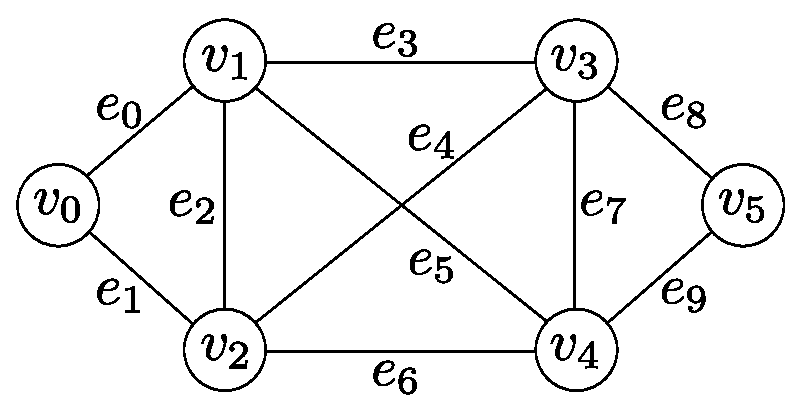
\includegraphics[scale=0.6]{figures/flownetwork.eps}
\caption{Flow network. $v_0$ is the source node and $v_5$ is the sink node.}
\label{fig:flownetwork}
\end{figure}

\subsubsection{Simple maximum flow case} \label{sec:maxflow}
Consider a case where our objective is to maximize the flow though the network, and each edge has a constant maximum capacity (see fig. \ref{fig:flownetwork_capacity}).

\begin{figure}[H]
\centering
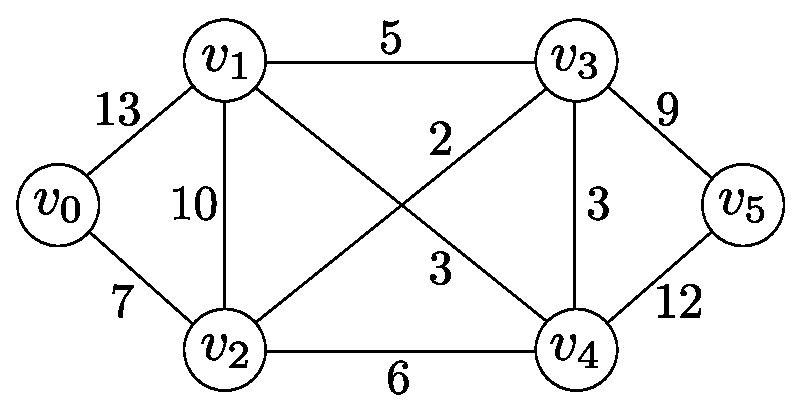
\includegraphics[scale=0.6]{figures/flownetwork_capacity.eps}
\caption{Flow network with constant capacities.}
\label{fig:flownetwork_capacity}
\end{figure}

The notation we will use is the following:
\begin{itemize}
\item
The flow through edge $e_j$ is $x_j$. Since the flows are our degrees of freedom, these are our optimization variables. We define our vector of optimization variables $x = [x_0, \dots, x_9]^\top$.
\item
The maximum flow, or capacity, for edge $e_j$ is $\overline{x}_j$. This gives us a vector of capacities $\overline{x} = [13, 7, 10, 5, 2, 3, 6, 3, 9, 12]^\top$. We also define $\underline{x} = -\overline{x}$, meaning the minimum flow is the negated maximum flow.
\end{itemize}

\paragraph{Incidence matrix.} To formulate the optimization problem, we will make use of an \emph{incidence matrix} $A = \lbrace a_{i,j} \rbrace$. The rows of the incidence matrix represent vertices, and the columns represent edges. If edge $j$ leaves vertex $i$, then $a_{i,j} = -1$. If edge $j$ enters vertex $i$, then $a_{i,j} = 1$. The incidence matrix for our flow network is shown below.
\[
\begin{array}{cc}
& 
e_0\ \ \ \ e_1\ \ \ \ e_2\ \ \ \ e_3\ \ \ \ e_4\ \ \ \ e_5\ \ \ \ e_6\ \ \ \ e_7\ \ \ \ e_8\ \ \ \ e_9
\\
\begin{array}{r}
v_0 \\ v_1 \\ v_2 \\ v_3 \\ v_4 \\ v_5
\end{array}
&
\left[
\begin{array}{cccccccccc}
-1 & -1 &  0 &  0 &  0 &  0 &  0 &  0 &  0 &  0 \\
 1 &  0 & -1 & -1 & -1 &  0 &  0 &  0 &  0 &  0 \\
 0 &  1 &  1 &  0 &  0 & -1 & -1 &  0 &  0 &  0 \\
 0 &  0 &  0 &  1 &  0 &  1 &  0 & -1 & -1 &  0 \\
 0 &  0 &  0 &  0 &  1 &  0 &  1 &  1 &  0 & -1 \\
 0 &  0 &  0 &  0 &  0 &  0 &  0 &  0 &  1 &  1 \\
\end{array}
\right]
\end{array}
= A
\]
Note that this incidence matrix could be slightly different since our flow network is undirected (liquid can flow both ways through a pipeline). However, here we have assumed that the default flow direction is right $\rightarrow$ left and up $\rightarrow$ down.

\paragraph{Optimization variables.} Our vector of optimization variables is $x = [x_0,\dots,x_9]^\top$, where $x_j$ is the flow through edge $e_j$.

\paragraph{Objective function.} We want to maximize the flow through the network. Another way of saying this is that we want to maximize the flow into the sink vertex $v_5$. This flow is the sum of the flows in edges $e_8$ and $e_9$, in other words, we want to maximize $x_8 + x_9$. This gives the linear objective
\[
\minimize \underbrace{\begin{bmatrix} 0 & 0 & 0 & 0 & 0 & 0 & 0 & 0 & -1 & -1 \end{bmatrix}}_{v^\top} \underbrace{\begin{bmatrix}x_0 \\ x_1 \\ x_2 \\ x_3 \\ x_4 \\ x_5 \\ x_6 \\ x_7 \\ x_8 \\ x_9 \end{bmatrix}}_x.
\]
Note that we could just as well have maximized the flow out of the source vertex, or the flow across any cut in the network.

\paragraph{Constraints.} We have two constraints; the mass balance constraint and the flow capacity constraint. We will implement the flow capacity constraint later when we define the variable bounds. The mass balance constraint says that for each vertex (except the source and the sink), the sum of inflows must equal the sum of outflows:
\[
\begin{array}{lr}
\mathrm{For\ vertex}\ v_1: & x_0 - x_2 - x_3 - x_4 = 0,\\
\mathrm{For\ vertex}\ v_2: & x_1 + x_2 - x_5 - x_6 = 0,\\
\mathrm{For\ vertex}\ v_3: & x_3 + x_5 - x_7 - x_8 = 0,\\
\mathrm{For\ vertex}\ v_4: & x_4 + x_6 + x_7 - x_9 = 0.\\
\end{array}
\]
To write this compactly, we define the matrix $A_{\mathrm{int}}$, which is the incidence matrix $A$ with the top and bottom rows removed (so that it represents only the internal nodes):
\[
A_{\mathrm{int}} = 
\begin{bmatrix}
 1 &  0 & -1 & -1 & -1 &  0 &  0 &  0 &  0 &  0 \\
 0 &  1 &  1 &  0 &  0 & -1 & -1 &  0 &  0 &  0 \\
 0 &  0 &  0 &  1 &  0 &  1 &  0 & -1 & -1 &  0 \\
 0 &  0 &  0 &  0 &  1 &  0 &  1 &  1 &  0 & -1 
 \end{bmatrix}.
\]
Now we can state the mass balance constraint as a linear system of equations $A_{\mathrm{int}}x = 0$. The source and sink vertices are assumed to have infinite capacity, so these are not represented in any constraints.

\paragraph{Variable bounds.} Since the optimization variables are the flows through the edges, we can represent the flow capacity constraints as bounds on the optimization variables:
\[
\underline{x} \leq x \leq \overline{x}.
\]
\paragraph{Optimization problem.} We now have the optimization problem
\begin{subequations}
\begin{align}
\minimize v^\top x \\
\subto A_{\mathrm{int}}x &= 0,\ \mathrm{(Mass\ balance)} \\
\underline{x} \leq x &\leq \overline{x}. \ \mathrm{(Flow\ capacity)}
\end{align}
\end{subequations}

\paragraph{Setting up and solving the problem.} We set up a new \class{TestProblem} class called \class{MaximumFlow}. The code below is implemented in the \texttt{solveProblem()} function to set up and solve the maximum flow problem.
\begin{lstlisting}[numbers=left]
void MaximumFlow::solveProblem()
{
    // Starting point: zero flow
    std::vector< double > z0 {0, 0, 0, 0, 0, 0, 0, 0, 0, 0};
    // Flow capacities (c)
    std::vector< double > lb
    		{-13,-7,-10,-5,-3,-2,-6,-3,-9,-12};
    std::vector< double > ub
    		{ 13, 7, 10, 5, 3, 2, 6, 3, 9, 12};
    // Incidence matrix
    DenseMatrix A(6, 10);
    A << -1, -1,  0,  0,  0,  0,  0,  0,  0,  0,
          1,  0, -1, -1, -1,  0,  0,  0,  0,  0,
          0,  1,  1,  0,  0, -1, -1,  0,  0,  0,
          0,  0,  0,  1,  0,  1,  0, -1, -1,  0,
          0,  0,  0,  0,  1,  0,  1,  1,  0, -1,
          0,  0,  0,  0,  0,  0,  0,  0,  1,  1;
    // Incidence matrix for internal nodes
    DenseMatrix A_int = A.block(1,0,4,10);
    // Objective function
    DenseMatrix v(1, 10);
    v << 0, 0, 0, 0, 0, 0, 0, 0, -1, -1;
    ObjectivePtr objective(new ObjectiveLinear(v));
    // Mass balance constraint
    DenseVector zeros; zeros.setZero(4,1);
    ConstraintPtr cMassBalance(new ConstraintLinear(A_int, zeros, true));
    // Constraint composite (with flow capacity as bounds)
    ConstraintCompositePtr constraints(new ConstraintComposite(10, lb, ub));
    constraints->add(cMassBalance);
    // Optimize
    OptimizerIpopt optIpopt(objective, constraints, z0);
    int status = optIpopt.optimize();
    fopt_found = optIpopt.getObjectiveValue();
    zopt_found = optIpopt.getOptimalSolution();
    cout << "Optimal solution: f*=" << fopt_found << endl;
    cout << "Optimal flows:" << endl;
    for (int i = 0; i < 10; i++) cout << "Edge " << i << ": " << zopt_found.at(i) << endl;
}
\end{lstlisting}
Line 4 defines the starting point, which we have chosen to be zero flow. Lines 6-9 define the variable bounds, which are also the edge capacities. Lines 10-19 define the incidence matrix and the internal node incidence matrix. Lines 20-23 define the objective function. Lines 24-26 define the mass balance constraint, and lines 27-29 define the constraint composite and adds the mass balance constraint. Lines 30-37 solves the problem and prints information about the solution. When used in the \class{TestProblem} framework, this gives us the following output:
\newline
{\footnotesize{\texttt{Running Maximum Flow problem...\\
\\
******************************************************************************\\
This program contains Ipopt, a library for large-scale nonlinear optimization.\\
 Ipopt is released as open source code under the Eclipse Public License (EPL).\\
         For more information visit http://projects.coin-or.org/Ipopt\\
******************************************************************************\\
\\
Optimal solution: f*=-16\\
Optimal flows:\\
Edge 0: 10.363\\
Edge 1: 5.63704\\
Edge 2: 2.36296\\
Edge 3: 5\\
Edge 4: 3\\
Edge 5: 2\\
Edge 6: 6\\
Edge 7: 0.196329\\
Edge 8: 6.80367\\
Edge 9: 9.19633\\
Maximum Flow problem successfully solved in 0 (ms)\\
Press <RETURN> to close this window...\\
}}}
We see that the four edges across the middle of the network are at full capacity, and it is not possible to increase the flow across this cut further, meaning this solution must be optimal (however, it is not the only optimal solution).

\begin{figure}[H]
\centering
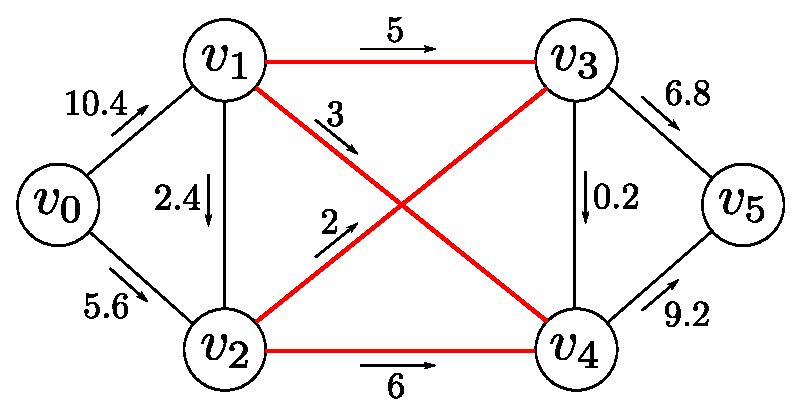
\includegraphics[scale=0.6]{figures/flownetwork_sol1.eps}
\caption{Optimal solution of maximum flow problem. Red edges indicate that the edge is at its maximum capacity.}
\label{fig:flownetwork_sol1}
\end{figure}

\subsubsection{Maximum flow with routing} \label{sec:maxflowrouting}
Now consider a case where we have to choose exactly two of the four edges across the network ($e_3$ - $e_6$). To do this, we introduce four new \emph{binary} optimization variables $b = [b_3,b_4,b_5,b_6]$ (we also augment $v$ with four zeros). When $b_j=1$, this means we allow flow through edge $e_j$, and when $b_j=0$, the flow through edge $e_j$ is locked to $x_j=0$. That is,
\[
x_j \in \left \lbrace \begin{array}{ll} [\underline{x}_j, \overline{x}_j], & b_j = 1, \\ \lbrace 0 \rbrace, & b_j = 0. \end{array} \right. 
\]
We can accomplish this by \emph{collapsing} the variable bounds based on the value of the binary variables. Consider the following:
\[
b_j\underline{x}_j \leq x_j \leq b_j\overline{x}_j.
\]
When $b_j = 1$, we have $\underline{x}_j \leq x_j \leq \overline{x}_j$ as usual. However, when $b_j = 0$, we have $0 \leq x_j \leq 0$, meaning we must have $x_j = 0$. This is called \emph{collapsing the bounds}. We can split this into two equations and write it on matrix form:
\begin{equation}
\begin{array}{rcl}
\begin{array}{r}
b_j \underline{x}_j - x_j \leq 0 \\
x_j - b_j \overline{x}_j \leq 0
\end{array}
&
\Rightarrow
&
\begin{bmatrix}
-1 & \underline{x}_j \\
1 & -\overline{x}_j
\end{bmatrix}
\begin{bmatrix} x_j \\ b_j \end{bmatrix}
\leq 0.
\end{array}
\label{eqn:routing}
\end{equation}
We want only two pipelines to be switched on, so we add the constraint
\begin{equation}
b_3 + b_4 + b_5 + b_6 = 2.
\label{eqn:numpipelines}
\end{equation}
Applying (\ref{eqn:routing}) to all four routing options and combining this with (\ref{eqn:numpipelines}), we get the linear inequality constraint
\[
\underbrace{\begin{bmatrix}
-1 & 0 & 0 & 0 & \underline{x}_3 & 0 & 0 & 0 \\
0 & -1 & 0 & 0 & 0 & \underline{x}_4 & 0 & 0 \\
0 & 0 & -1 & 0 & 0 & 0 & \underline{x}_5 & 0 \\
0 & 0 & 0 & -1 & 0 & 0 & 0 & \underline{x}_6 \\
1 & 0 & 0 & 0 & -\overline{x}_3 & 0 & 0 & 0 \\
0 & 1 & 0 & 0 & 0 & -\overline{x}_4 & 0 & 0 \\
0 & 0 & 1 & 0 & 0 & 0 & -\overline{x}_5 & 0 \\
0 & 0 & 0 & 1 & 0 & 0 & 0 & -\overline{x}_6 \\
0 & 0 & 0 & 0 & 1 & 1 & 1 & 1 \\
0 & 0 & 0 & 0 & -1 & -1 & -1 & -1 \\
\end{bmatrix}}_{A_R}
\underbrace{\begin{bmatrix}
x_3 \\ x_4 \\ x_5 \\ x_6 \\ b_3 \\ b_4 \\ b_5 \\ b_6
\end{bmatrix}}_{\tilde{x}}
\leq
\underbrace{\begin{bmatrix}
0 \\ 0 \\ 0 \\ 0 \\ 0 \\ 0 \\ 0 \\ 0 \\ 2 \\ -2
\end{bmatrix}}_{b_R}
\]

\paragraph{Optimization problem.} Our new optimization problem becomes
\begin{subequations}
\begin{align}
\minimize v^\top \begin{bmatrix} x \\ b \end{bmatrix} \\
\subto A_{\mathrm{int}}x &= 0,\ \mathrm{(Mass\ balance)} \\
A_R \tilde{x} &\leq b_R,\ \mathrm{(Routing)} \label{eqn:routingconstr}\\
\underline{x} \leq x &\leq \overline{x}.\ \mathrm{(Flow\ capacity)}
\end{align}
\end{subequations}

\paragraph{Setting up and solving the problem.} We set up a new \class{TestProblem} class called \class{FlowWithRouting}. The code below is implemented in the \texttt{solveProblem()} function to set up and solve the flow problem with routing constraints.
\begin{lstlisting}[numbers=left]
void FlowWithRouting::solveProblem()
{
    // Starting point: zero flow
    std::vector< double > z0 {0, 0, 0, 0, 0, 0, 0, 0, 0, 0, 0, 0, 0, 0};
    // Flow capacities (c)
    std::vector< double > lb {-13, -7, -10, -5, -3, -2, -6, -3, -9, -12, 0, 0, 0, 0};
    std::vector< double > ub { 13,  7,  10,  5,  3,  2,  6,  3,  9,  12, 1, 1, 1, 1};
    // Incidence matrix
    DenseMatrix A(6, 10);
    A << -1, -1,  0,  0,  0,  0,  0,  0,  0,  0,
          1,  0, -1, -1, -1,  0,  0,  0,  0,  0,
          0,  1,  1,  0,  0, -1, -1,  0,  0,  0,
          0,  0,  0,  1,  0,  1,  0, -1, -1,  0,
          0,  0,  0,  0,  1,  0,  1,  1,  0, -1,
          0,  0,  0,  0,  0,  0,  0,  0,  1,  1;
    // Incidence matrix for internal nodes
    DenseMatrix A_int = A.block(1,0,4,10);
    // Objective function
    DenseMatrix v(1, 14);
    v << 0, 0, 0, 0, 0, 0, 0, 0, -1, -1, 0, 0, 0, 0;
    ObjectivePtr objective(new ObjectiveLinear(v));
    // Mass balance constraints
    std::vector< int > massBalanceVars {0,1,2,3,4,5,6,7,8,9};
    VecD zeros4; zeros4.setZero(4, 1);
    ConstraintPtr cMassBalance(new ConstraintLinear(A_int, zeros4, true));
    // Routing constraints
    DenseMatrix AR(10, 8);
    AR << -1, 0, 0, 0, lb.at(3),        0,        0,        0,
           0,-1, 0, 0,        0, lb.at(4),        0,        0,
           0, 0,-1, 0,        0,        0, lb.at(5),        0,
           0, 0, 0,-1,        0,        0,        0, lb.at(6),
           1, 0, 0, 0,-ub.at(3),        0,        0,        0,
           0, 1, 0, 0,        0,-ub.at(4),        0,        0,
           0, 0, 1, 0,        0,        0,-ub.at(5),        0,
           0, 0, 0, 1,        0,        0,        0,-ub.at(6),
           0, 0, 0, 0,        1,        1,        1,        1,
           0, 0, 0, 0,       -1,       -1,       -1,       -1;
    VecD bR; bR.setZero(10, 1);
    bR(8) = 2;
    bR(9) = -2;
    // Variables x3-x6 and b3-b6
    std::vector< int > routingVars {3,4,5,6,10,11,12,13};
    ConstraintPtr cRouting(new ConstraintLinear(AR,bR,false));
    // Constraint composite (with flow capacity as bounds)
    ConstraintCompositePtr constraints(new ConstraintComposite(14, lb, ub));
    constraints->add(cMassBalance, massBalanceVars);
    constraints->add(cRouting, routingVars);
    // Variable types
    std::vector< int > variable_types;
    for (int i = 0; i < 10; i ++) variable_types.push_back(CONTINUOUS);
    for (int i = 0; i < 4; i ++) variable_types.push_back(BINARY);
    // Branching variables (routing options)
    std::vector< int > branching_variables {10, 11, 12, 13};
    // Optimize
    BranchAndBound bnb(objective, constraints, z0, variable_types, branching_variables);
    int status = bnb.optimize();
    fopt_found = bnb.getObjectiveValue();
    zopt_found = bnb.getOptimalSolution();
    cout << "Optimal solution: f*=" << fopt_found << endl;
    cout << "Optimal flows:" << endl;
    for (int i = 0; i < 10; i++) cout << "Edge " << i << ": " << zopt_found.at(i) << endl;
    cout << "Routing decision:" << endl;
    for (int i = 10; i < 14; i++) cout << "Edge " << i-7 << ": " << zopt_found.at(i) << endl;
}
\end{lstlisting}
The differences between this and the previous example is the following:
\begin{itemize}
\item
Lines 3-7: Starting point and bound vectors are augmented with four elements to facilitate the new routing variables.
\item
Line 23: We have defined variable mapping vector for the mass balance constraints, since this constraint no longer includes all the variables.
\item
Lines 27-42 is the implementation of equation (\ref{eqn:routingconstr}); that is, the routing constraints.
\item
Lines 45-46 add both constraint pointers to the constraint composite (in the previous example only one constraint pointer was added).
\item
Lines 47-50 define the variable types; variables 0 to 9 ($x_0$-$x_9$) are continuous, while variables 10 to 13 ($b_3$-$b_6$) are binary.
\item
Line 52 define the branching variables; these are the binary variables $b_3$-$b_6$.
\item
Lines 54-55: We use the \class{BranchAndBound} solver in stead of \class{OptimizerIpopt}, since we have a MILP with integer variables which cannot be solved directly in Ipopt.
\end{itemize}
This code gives the output
\newline
{\footnotesize{\texttt{Optimal solution: f*=-11 \\
Optimal flows: \\
Edge 0: 7.526\\
Edge 1: 3.474\\
Edge 2: 2.526\\
Edge 3: 5\\
Edge 4: 0\\
Edge 5: 1.957e-08\\
Edge 6: 6\\
Edge 7: 0.2101\\
Edge 8: 4.79\\
Edge 9: 6.21\\
Routing decision:\\
Edge 3: 1\\
Edge 4: 0\\
Edge 5: 0\\
Edge 6: 1\\
Maximum Flow with Routing problem successfully solved in 370 (ms)\\
Press <RETURN> to close this window...\\
}}}
This solution is shown graphically in fig. \ref{fig:flownetwork_sol2}. As expected, the two edges with the largest capacity are selected and the maximum flow is 11.
\begin{figure}[H]
\centering
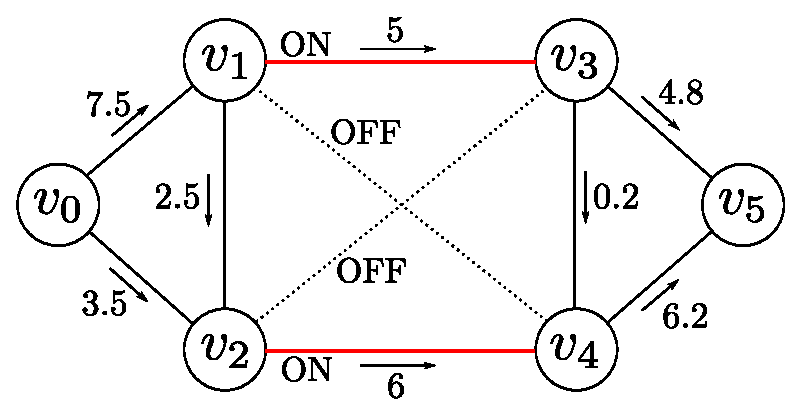
\includegraphics[scale=0.6]{figures/flownetwork_sol2.eps}
\caption{Optimal solution of maximum flow problem with routing constraints. Red edges indicate that the edge is at its maximum capacity and dotted lines indicate that they have been swithced off.}
\label{fig:flownetwork_sol2}
\end{figure}

\paragraph{Integer variables.} \label{sec:maxflowinteger} If we want a solution with integer flows, this is easily achieved by specifying $x_0$-$x_9$ as integer variables and adding them as branching variables in lines 48-53:
\begin{lstlisting}
// Variable types
    std::vector< int > variable_types;
    for (int i = 0; i < 10; i ++) variable_types.push_back(INTEGER);
    for (int i = 0; i < 4; i ++) variable_types.push_back(BINARY);
    // Branching variables (routing options)
    std::vector< int > branching_variables {0,1,2,3,4,5,6,7,8,9,10,11,12,13};
\end{lstlisting}
This gives the solution shown in fig. \ref{fig:flownetwork_sol3}.
\begin{figure}[H]
\centering
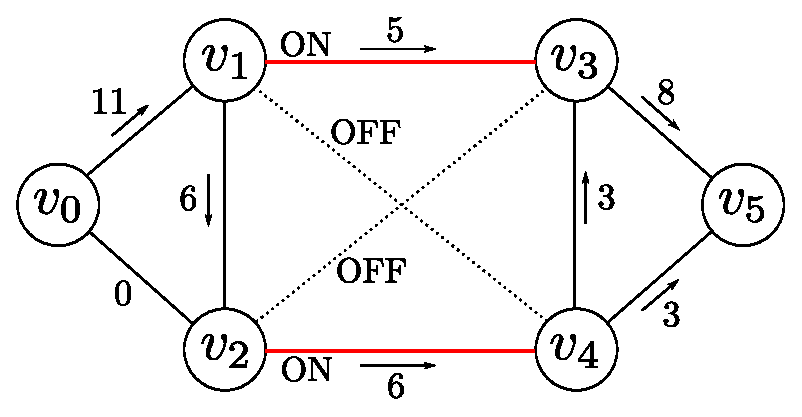
\includegraphics[scale=0.6]{figures/flownetwork_sol3.eps}
\caption{Optimal solution of maximum flow problem with routing constraints and integer variables.}
\label{fig:flownetwork_sol3}
\end{figure}

\subsubsection{Pressure driven flow case - Linear flow model {\color{red} (INCOMPLETE)}}
Now we will augment the network model to include pressure/potential. We assume a constant pressure in the source vertex, and a constant pressure in the sink vertex. Given a set of equations which describe the pressure drop across each edge/pipeline, we can formulate a maximum flow problem which takes into account the pressure loss in the pipelines. For this example, we assume the flow $x_j$ through edge $e_j$ is given by
\[
x_j = f(p_A, p_B),
\]
where $p_A$ is the pressure in the start vertex and $p_B$ is the pressure in the end vertex (see fig. \ref{fig:pressuredrop})
\begin{figure}[H]
\centering
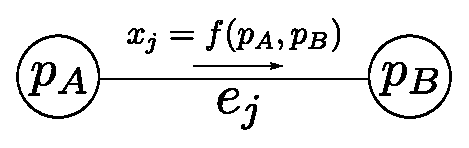
\includegraphics[scale=0.6]{figures/pressuredrop.eps}
\caption{Flow model.}
\label{fig:pressuredrop}
\end{figure}
In this section, we will assume a simple model where the flow is a linear function of the pressure drop, that is,
\[
f(p_A, p_B) = k(p_A - p_B).
\]

\paragraph{Optimization variables.} We have to add the pressures in each vertex to the vector of optimization variables. Our new vector of optimization variables is $[x^\top,p^\top]^\top = [x_0,\dots,x_9,p_0,\dots,p_5,b_3,\dots b_6]^\top$, where $p_i$ is the pressure in vertex $v_i$.

\paragraph{Objective function.} The objective function is the same as in the previous example, but we must augment $v$ with six zeros to facilitate the new optimization variables: $v = [0,0,0,0,0,0,0,0,-1,-1,0,0,0,0,0,0, 0, 0, 0, 0]^\top$.

\paragraph{Constraints.} We keep the mass balance $A_{\mathrm{int}}x=0$, and add the flow equation constraints
\begin{align*}
x_0 &= k_0(p_0 - p_1) \\
x_1 &= k_1(p_0 - p_2) \\
x_2 &= k_2(p_1 - p_2) \\
x_3 &= k_3(p_1 - p_3) \\
x_4 &= k_4(p_1 - p_4) \\
x_5 &= k_5(p_2 - p_3) \\
x_6 &= k_6(p_2 - p_4) \\
x_7 &= k_7(p_3 - p_4) \\
x_8 &= k_8(p_3 - p_5) \\
x_9 &= k_9(p_4 - p_5). \\
\end{align*}
We can make use of our incidence matrix and collect the $k_j$'s in a diagonal matrix $K = \mathrm{diag}\ \lbrace k_0, \dots, k_9 \rbrace$, and write this as $-K A^\top p = x$ (we leave it to the reader to verify this), which gives us the constraint
\[
\begin{bmatrix}  -I & -K A^\top \end{bmatrix} \begin{bmatrix} x \\ p \end{bmatrix} = 0.
\]

\paragraph{Variable bounds.} We keep the flow capacity constraints as bounds on $x$ and let the pressures in the internal vertices be unbounded. However, we want constant pressures in the source vertex and the sink vertex. We let the pressure in the source be 10, and demand the pressure in the sink be greater than 0. This is accomplished by using the upper and lower bounds for these two pressures.

\paragraph{Optimization problem.} We now have the optimization problem
\begin{subequations}
\begin{align}
\minimize v^\top \begin{bmatrix} x \\ p \\ b\end{bmatrix} \\
\subto A_{\mathrm{int}}x &= 0,\ \mathrm{(Mass\ balance)} \\
A_R \tilde{x} &\leq b_R,\ \mathrm{(Routing)} \\
\begin{bmatrix} -I & -K A^\top \end{bmatrix} \begin{bmatrix} x \\ p \end{bmatrix} &= 0,\ \mathrm{(Flow\ equations)} \\
-c \leq x &\leq c,\ \mathrm{(Flow\ capacity)} \\
10 \leq p_0 &\leq 10,\ \mathrm{(Source\ pressure)}\\
0 \leq p_5 &\leq \infty.\ \mathrm{(Sink\ pressure)}
\end{align}
\end{subequations}


\newpage
\subsection{The Six-Hump Camelback function}
In this section we will minimize the Six-Hump Camelback function locally and globally, using various methods. The Six-Hump Camelback function is a classical test function for optimization algorithms, and is found many places in the literature. The function has two variables, and is given by
\begin{equation}
f_{\mathrm{SH}}(x_0, x_1) = \left( 4 - 2.1x_0^2 + \frac{x_0^4}{3} \right)x_0^2 + x_0x_1 + (-4 + 4x_1^2) x_1^2.
\label{eqn:schb}
\end{equation}
The interesting area of this function is in the domain given by $-3 \leq x_0 \leq 3$ and $-2 \leq x_1 \leq 2$. Within this domain, there are six local minima, two of which are global minima. The global minimum is $f_{\mathrm{SH}}^* = f_{\mathrm{SH}}(x_0^*, x_1^*) = -1.0316$ at $(x_0^*, x_1^*) = (-0.0898, 0.7126)$ and $(0.0898, -0.7126)$.
\begin{figure}[H]
\centering
\subfigure[$-3 \leq x_0 \leq 3$ and $-2 \leq x_1 \leq 2$]{
	\includegraphics[scale=0.45]{figures/shcb_low.eps} 
	\label{fig:shcb1}
}
\subfigure[A closer look: $-2 \leq x_0 \leq 2$ and $-1 \leq x_1 \leq 1$]{
	\includegraphics[scale=0.45]{figures/shcb_zoom_low.eps} 
	\label{fig:shcb2}
}
\caption{The Six-Hump Camelback function.}
\end{figure}

\subsubsection{Formulating the optimization problem}
We want to find the global minimum of the Six-Hump Camelback function, that is, we want to solve the unconstrained optimization problem
\begin{equation}
\minimize x_2 = \left( 4 - 2.1x_0^2 + \frac{x_0^4}{3} \right)x_0^2 + x_0x_1 + (-4 + 4x_1^2) x_1^2
\label{eqn:shcb_orig}
\end{equation}
Note that we have introduced the new variable $x_2 = f_{\mathrm{SH}}(x_0, x_1)$. The reason for this is that we want to state (\ref{eqn:shcb_orig}) in its epigraph form (see section \ref{sec:epigraph}). We define a vector of optimization variables $x = [x_0, x_1, x_2]^\top$. Since we want to minimize $x_2$, this gives the linear objective function
\begin{equation}
f(x) = \begin{bmatrix} 0 & 0 & 1 \end{bmatrix} \begin{bmatrix} x_0 \\ x_1 \\ x_2 \end{bmatrix} = v^\top x.
\label{eqn:shcb_linobj}
\end{equation}
We want to restrict $x_2$ to the epigraph of $f_{\mathrm{SH}}$, so we add the constraint $x_2 \geq f_{\mathrm{SH}}(x_0, x_1)$, which is equivalent to $f_{\mathrm{SH}}(x_0, x_1) - x_2 \leq 0$. Since we want both an upper and lower bound on our constraint function, we add the lower bound $-\infty$ and end up with the reformulated optimization problem
\begin{subequations}
\begin{align}
\minimize f(x) &= v^\top x \\
\subto -\infty &\leq c_1(x_0, x_1, x_2) = f_{\mathrm{SH}}(x_0, x_1) - x_2 \leq 0. \label{eqn:shcb_reform_constr}
\end{align}
\end{subequations}
Note that setting the lower bound equal to zero would give the same solution; this would restrict $x_2$ to lie \emph{on} the graph of $f_{\mathrm{SH}}$ as opposed to \emph{on or above} the graph of $f_{\mathrm{SH}}$.

\subsubsection{Domain bounds, starting point, objective function and constraint set.} Defining the variable domain bounds,  starting point, objective function and constraint set will be the same for all the different approaches below, so we will start with these.

\paragraph{Define domain bounds.} First, we define our domain bounds. We have restricted $x_0$ to $\pm 3$ and $x_1$ to $\pm2$, while $x_2$ is our free variable and should be unrestricted ($\pm \infty$). The domain bounds are defined using vectors of doubles which are passed to the constraint composite (see section \ref{sec:constraintcomposite}).
\begin{lstlisting}
std::vector<double> lb;	// Lower bound
std::vector<double> ub;	// Upper bound

lb.push_back(-3);		// Lower bound for x0
lb.push_back(-2);		// Lower bound for x1
lb.push_back(-IPOPT_UNBOUNDED);	// Lower bound for x2

ub.push_back(3);		// Upper bound for x0
ub.push_back(2);		// Upper bound for x1
ub.push_back(IPOPT_UNBOUNDED);	// Upper bound for x2
\end{lstlisting}

\paragraph{Define the starting point.} The starting point for the optimization is also defined using a vector of doubles. Since we are solving the problem locally, the starting point will affect which solution we end up with. When following this example, the reader should experiment with several different starting points to see how the solver behaves.
\begin{lstlisting}
std::vector<double> z0;	// Starting point

z0.push_back(0);	// Starting point, x0 coordinate
z0.push_back(0);	// Starting point, x1 coordinate
z0.push_back(0);	// Starting point, x2 coordinate
\end{lstlisting}

\paragraph{Define the objective function.} The objective function  is defined using the \class{ObjectiveLinear} class (since we have a linear objective function). The constructor for this class takes an Eigen matrix as an input parameter, which is the vector $v$ from (\ref{eqn:shcb_linobj}):
\begin{lstlisting}
int numVars = 3;	// Number of variables (x0, x1 and x2)
DenseMatrix v(1,numVars); // 1 x 3 matrix (row vector)
v << 0, 0, 1;		// Fill v with values
// Create the objective object
ObjectivePtr objective (new ObjectiveLinear(v));
\end{lstlisting}

\paragraph{Create a \class{ConstraintComposite} object.} To create the \class{ConstraintComposite} object, we need the number of variables, and the upper and lower bounds for these variables. These were defined above, so we can proceed with creating a constraint composite to which we can add constraints later.
\begin{lstlisting}
ConstraintCompositePtr constraints(new ConstraintComposite(numVars, lb, ub));
\end{lstlisting}
\subsubsection{Local optimization using the \class{ConstraintPolynomial} class} \label{sec:shcb_polynomial}
Note that $f_{\mathrm{SH}}$ can be written as a sum of monomial terms:
\[
f_{\mathrm{SH}}(x_0, x_1) = \frac{x_0^6}{3} - 2.1 x_0^4 + 4x_0^2 + x_0 x_1 + 4x_1^4-4x_1^2.
\]
This means we can write (\ref{eqn:shcb_reform_constr}) on the form (\ref{eqn:polyconstr}) and implement the Six-Hump Camelback function as a polynomial constraint. First, we need to find the vector $c$ and the matrix $E$ used in (\ref{eqn:polyconstr}). We have that
\begin{align*}
&\frac{x_0^6}{3} - 2.1 x_0^4 + 4x_0^2 + x_0 x_1 + 4x_1^4-4x_1^2 - x_2 \\
&= \frac{1}{3}x_0^6 x_1^0 x_2^0 -2.1 x_0^4 x_1^0 x_2^0 + 4x_0^2 x_1^0 x_2^0 \\
&+ x_0^1 x_1^1 x_2^0 + 4x_0^0 x_1^4 x_2^0 - 4x_0^0  x_1^2 x_2^0 - x_0^0 x_1^0 x_2^1,
\end{align*}
so we get
\begin{equation}
c = \begin{bmatrix} \frac{1}{3} \\ -2.1 \\ 4 \\ 1 \\ 4 \\ -4 \\ -1 \end{bmatrix}\ \ \ \mathrm{and}\ \ \ E = \begin{bmatrix} 6 & 0 & 0 \\ 4 & 0 & 0 \\ 2 & 0 & 0 \\ 1 & 1 & 0 \\ 0 & 4 & 0 \\ 0 & 2 & 0 \\ 0 & 0 & 1 \end{bmatrix}.
\label{eqn:candE}
\end{equation}
We are now ready to solve the optimization problem using \solvername. To do this, we complete the following steps:
\begin{itemize}
\item Add the constraint header file
\item Define the Six-Hump Camelback constraint
\item Add the constraint to the constraint composite
\item Solve the optimization problem with a local solver
\end{itemize}

\paragraph{Add the constraint header file.} The first thing we must do is to include the \class{ConstraintPolynomial} header file, since we will be using this class to define our constraint.
\begin{lstlisting}
#include "OptimizationProblem/constraintpolynomial.h"
\end{lstlisting}

\paragraph{Define the Six-Hump Camelback constraint.} As mentioned above, we will use the \class{ConstraintPolynomial} class to define the Six-Hump Camelback function using the vector $c$ and the matrix $E$ from (\ref{eqn:candE}). $c$ must be defined as an Eigen vector and $E$ must be defined as an Eigen matrix:
\begin{lstlisting}
DenseVector c(7);		// 7 X 1 Eigen vector
DenseMatrix E(7, 3);	// 7 X 3 Eigen matrix

// Fill c and E with values using the << operator
c << (1/3.0), -2.1, 4, 1, 4, -4, -1;
E <<	6, 0, 0,
		4, 0, 0,
		2, 0, 0,
		1, 1, 0,
		0, 4, 0,
		0, 2, 0,
		0, 0, 1;
\end{lstlisting}
Now we can create the \class{ConstraintPolynomial} object. The third and fourth parameters passed to the constructor are the constraint's lower and upper bound from (\ref{eqn:shcb_reform_constr}), which are $-\infty$ and $0$, respectively.
\begin{lstlisting}
ConstraintPtr cSixHump(new ConstraintPolynomial(c, E, -IPOPT_UNBOUNDED, 0));
\end{lstlisting}

\paragraph{Add the constraint to the \class{ConstraintComposite} object.} Now that we have defined a constraint object, we need to add this to the \class{ConstraintComposite} object that we created earlier. To do this, we have to define a variable mapping to tell the \class{ConstraintComposite} object which variables are present in the constraint being added. In this case, all the variables ($x_0$, $x_1$ and $x_2$) are present, so we create a vector of integers which contains the indices of each variable (0, 1 and 2):
\begin{lstlisting}
std::vector<int> variableMapping;
variableMapping.push_back(0);
variableMapping.push_back(1);
variableMapping.push_back(2);
\end{lstlisting}
When this vector of integers is passed to the constraint composite object, we are telling it that variable 0 in the constraint composite corresponds to variable 0 in the polynomial constraint that is being added, and the same goes for variables 1 and 2. Now that the variable mapping vector has been created, we are ready to add our constraint to the constraint composite:
\begin{lstlisting}
constraints->add(cSixHump, variableMapping);
\end{lstlisting}

\paragraph{Solve the optimization problem with a local solver.} Since we do not yet have a convex relaxation of our constraint available, we are only able to solve the optimization problem locally. Now that we have defined our objective object, constraint composite object and starting point, \solvername\ provides a sleek interface to Ipopt for solving optimization problems locally. All that is required is to create an object of type \class{OptimizerIpopt} with our objective, constraints and starting point, and call its \texttt{optimize()} function:
\begin{lstlisting}
OptimizerIpopt optIpopt(objective, constraints, z0);
int status = optIpopt.optimize();
\end{lstlisting}
We can also output some information about the solution obtained:
\begin{lstlisting}
cout << "Solved (locally) using Ipopt!" << endl;
cout << "Status: " << status << endl;
cout << "f*: " << optIpopt.getObjectiveValue() << endl;
cout << "x*: ";
printVec(optIpopt.getOptimalSolution());
\end{lstlisting}
With the starting point $z_0 = (0, 0, 0)$, we should get the following output:
\texttt{
Solved (locally) using Ipopt! \\
Status: 1 \\
f*: -9.99e-09 \\
x*: (     0,      0,      0)} \\
This is not the global optimum; Ipopt is stuck in the saddle point located at the origin. However, if we try different starting points, we will obtain better solutions. For instance, if we give Ipopt the starting point $z_0 = (1, 0, 0)$, it finds the global minimum at $x^* = (0.08984, -0.7127, -1.032)$, and the starting point $z_0 = (-1, 0, 0)$ gives the other globally optimal point at $x^* = (-0.08984, 0.7127, -1.032)$.

\subsubsection{Local optimization using a custom constraint class} \label{sec:shcb_custom}
What if our constraint does not fit into the \class{ConstraintPolynomial} class or any of the other contstraint classes provided? In this case, we must create a custom constraint class which inherits from the \class{Constraint} class. If we take a look in the header file of this class, we see that quite a few of the public functions are declared \keyword{virtual}. These functions must be implemented in any class which inherits from the \class{Constraint} class. We will create a new class which inherits from \class{Constraint} and call it \class{ConstraintSixHumpCamel}. We start off with the header file \texttt{constraintsixhumpcamel.h}:
\begin{lstlisting}
#ifndef CONSTRAINTSIXHUMPCAMEL_H
#define CONSTRAINTSIXHUMPCAMEL_H
#include "constraint.h"

class ConstraintSixHumpCamel : public Constraint
{
public:
    ConstraintSixHumpCamel();
};
#endif // CONSTRAINTSIXHUMPCAMEL_H
\end{lstlisting}
We will now complete the following steps to implement this constraint class and solve the optimization problem:
\begin{itemize}
\item Implement the constructor
\item Implement the clone function
\item Implement the function evaluation
\item Implement the Jacobian evaluation
\item Implement the Hessian evaluation
\item Define the structure of the Jacobian
\item Define the structure of the Hessian
\item Create an instance of the constraint
\item Add the constraint to the constraint composite
\item Run the optimization problem
\end{itemize}

\paragraph{Implementing the constructor.} In the constructor, we must set some constraint properties that are used for various checks. The most basic properties we must set are
\begin{itemize}
\item
The number of variables (the dimension of the constraint's domain).
\item
The number of outputs. If there are several equations in one constraint class this number may be different than 1, but in this case there is only one equation.
\item
The domain bounds of the variables.
\item
The domain bounds of the output(s).
\item
Basic constraint properties:
\begin{itemize}
\item Is the Jacobian calculated?
\item Is the Hessian calculated?
\item Is the constraint linear?
\item Is the constraint convex?
\item Is there a convex relaxation available?
\end{itemize}
\item
The number of nonzero elements in the Jacobian.
\item
The number of nonzero elements in the Hessian.
\end{itemize}
We implement the following constructor:
\begin{lstlisting}
ConstraintSixHumpCamel::ConstraintSixHumpCamel()
{
	// Dimension of domain and codomain 
	dimensionDomainF = 3;
	dimensionCodomainF = 1;
	// Set the variable bounds to be unbounded
	setDomainBoundsUnbounded();
	// Set the output bounds between -Inf and 0
	lowerBoundF.push_back(-IPOPT_UNBOUNDED);
	upperBoundF.push_back(0);
	// Gradient: true, Hessian: true, Linear: false, Convex: false, Convex relaxation: false
	setConstraintProperties(true,true,false,false,false);
	// Number of nonzero elements in the Jacobian and Hessian
	nnzGradient = 3;
	nnzHessian  = 3;
	// Check settings for obvious mistakes
	checkConstraintSanity();
}
\end{lstlisting}

\paragraph{Implementing the clone function.} When a constraint is added to a constraint composite, what actually happens is that a copy of the constraint is created by calling the desired constraint class \texttt{clone()} function. Therefore, we must implement the \texttt{clone()} function here. This function simply returns a pointer to a clone of the constraint which is created by the copy constructor, which is a built-in function that creates a new object and copies all the values of each data member from the original to the copy. We implement it directly in the header file:
\begin{lstlisting}
virtual ConstraintSixHumpCamel* clone() const {return new ConstraintSixHumpCamel(*this);}
\end{lstlisting}

\paragraph{Implementing the function evaulation.} In the function evaluation function, we simply implement the function given by (\ref{eqn:shcb_reform_constr}). We add the declaration as a public function in the header file:
\begin{lstlisting}
public:
	virtual void evalF(DenseVector & x,DenseVector & y);
\end{lstlisting}
The parameters of the function are
\begin{itemize}
\item
\texttt{x}, which is an Eigen vector of doubles with the values of each variable.
\item
\texttt{y}, which is also an Eigen vector of doubles where we write the function value evaluated at \texttt{x}.
\end{itemize}
Recall that we wish to evaluate the function
\[
c_1(x_0, x_1, x_2) = \left( 4 - 2.1x_0^2 + \frac{x_0^4}{3} \right)x_0^2 + x_0x_1 + (-4 + 4x_1^2) x_1^2 - x_2.
\]
We implement the function in the .cpp file:
\begin{lstlisting}
void ConstraintSixHumpCamel::evalF(DenseVector & x,DenseVector & y)
{
	double t1 = (4.0-2.1*pow(x(0),2)+pow(x(0),4)/3.0);
	double t2 = -4+4*pow(x(1),2);

	y(0) = t1*pow(x(0),2)+x(0)*x(1)+t2*pow(x(1),2)-x(2);
}
\end{lstlisting}
Here, the doubles \texttt{t1} and \texttt{t2} are only used as temporary storage to make the expression for \texttt{y(0)} a little bit tidier.

\paragraph{Implementing the Jacobian evaulation.} To implement the Jacobian evaulation, we must first calculate the Jacobian. The Jacobian $\nabla c_1(x)$ is
\begin{align*}
\nabla c_1(x) &= \begin{bmatrix} \frac{\partial c_1}{\partial x_0}, & \frac{\partial c_1}{\partial x_1}, & \frac{\partial c_1}{\partial x_2} \end{bmatrix} \\
&= \begin{bmatrix} 8x_0 - 8.4x_0^3 + 2x_0^5 + x_1, & x_0 - 8x_1 + 16x_1^3, & -1 \end{bmatrix}.
\end{align*}
When implementing the Jacobian evaluation function, the value of \texttt{nnzGradient} defines the number of elements we must calculate. This value was set to three because there are three nonzero elements in the Jacobian. We add the declaration as a public function in the header file:
\begin{lstlisting}
public:
	virtual void evalGradF(DenseVector & x,DenseVector & dx);
\end{lstlisting}
The parameters of the function are
\begin{itemize}
\item
\texttt{x}, which is an Eigen vector of doubles with the values of each variable.
\item
\texttt{dx}, which is also an Eigen vector of doubles where we write the value of the Jacobian elements evaluated at \texttt{x}.
\end{itemize}
We implement the function in the .cpp file:
\begin{lstlisting}
void ConstraintSixHumpCamel::evalGradF(DenseVector & x,DenseVector & dx)
{
	dx(0) = 8*x(0)-8.4*pow(x(0),3)+2*pow(x(0),5)+x(1);
	dx(1) = x(0)-8*x(1)+16*pow(x(1),3);
	dx(2) = -1;
}
\end{lstlisting}
An important remark here is that \texttt{dx(0)} does not necessarily mean the first element of the Jacobian; we will later implement the function \texttt{structureGradF}, which maps each element of \texttt{dx} to the correct element in the Jacobian.

\paragraph{Implementing the Hessian evaluation.} We calculate the Hessian $\nabla^2 c_1(x)$:
\begin{equation}
\nabla^2 c_1(x) = \begin{bmatrix} 8 - 25.2x_0^2 + 10x_0^4 & 1 & 0 \\ 1 & 48x_1^2 - 8 & 0 \\ 0 & 0 & 0 \end{bmatrix} \label{eqn:shcb_hessian}
\end{equation}
This Hessian has three nonzero elements, which is the reason we set \texttt{nnzHessian} to 3 in the constructor. Although there are technically four nonzero elements, we do not count the symmetric elements of the Hessian, since these are redundant. We add the declaration as a public function in the header file:
\begin{lstlisting}
public:
	virtual void evalHessianF(DenseVector& x,DenseVector & ddx);
\end{lstlisting}
The parameters of the function are
\begin{itemize}
\item
\texttt{x}, which is an Eigen vector of doubles with the values of each variable.
\item
\texttt{ddx}, which is also an Eigen vector of doubles where we write the value of the Hessian elements evaluated at \texttt{x}.
\end{itemize}
We implement the function in the .cpp file:
\begin{lstlisting}
void ConstraintSixHumpCamel::evalHessianF(DenseVector& x,DenseVector & ddx)
{
	ddx(0) = 8-25.2*pow(x(0),2)+10*pow(x(0),4);
    ddx(1) = 1;
    ddx(2) = 48*pow(x(1),2)-8;
}
\end{lstlisting}
As with the Jacobian, the elements of \texttt{ddx} contain the values of the nonzero elements, and we will define the position of these elements later in the function \texttt{structureHessianF}.

\paragraph{Defining the structure of the Jacobian.} Next, we will implement the function \texttt{structureGradF}, which defines the position of the nonzero elements in the Jacobian. We add the declaration as a public function in the header file:
\begin{lstlisting}
public:
	virtual void structureGradF(std::vector< int >& iRow, std::vector< int >& jCol);
\end{lstlisting}
The parameters of the function are
\begin{itemize}
\item
\texttt{iRow}, which is an STL vector of integers with the row indices of the elements of \texttt{dx}.
\item
\texttt{jCol}, which is an STL vector of integers with the column indices of the elements of \texttt{dx}.
\end{itemize}
In our case, the calculated values assume the following positions in the Jacobian:
\[
\begin{array}{l|c|c|c|}
& \mathrm{Col\ 0} & \mathrm{Col\ 1} & \mathrm{Col\ 2} \\
\hline
\mathrm{Row\ 0} & \mathtt{dx(0)} & \mathtt{dx(1)} & \mathtt{dx(2)} \\
\hline
\end{array}
\]
That is, the value calculated for \texttt{dx(0)} should be placed in the (0,0) element of the Jacobian, \texttt{dx(1)} should be placed in the (0,1) element and \texttt{dx(2)} should be placed in the (0,2) element. This gives the following implementation in the .cpp file:
\begin{lstlisting}
void ConstraintSixHumpCamel::structureGradF(std::vector< int > &iRow, std::vector< int > &jCol)
{
	// Position of dx(0) is (0,0)
	iRow.push_back(0); jCol.push_back(0);
	// Position of dx(1) is (0,1)
	iRow.push_back(0); jCol.push_back(1);
	// Position of dx(2) is (0,2)
	iRow.push_back(0); jCol.push_back(2);
}
\end{lstlisting}

\paragraph{Defining the structure of the Hessian.}
The function \texttt{structureHessianF} defines the position of the nonzero elements in the Hessian. We add the declaration as a public function in the header file:
\begin{lstlisting}
public:
	virtual void structureHessianF(std::vector< int >& eqnr,std::vector< int >& iRow, std::vector< int >& jCol);
\end{lstlisting}
The parameters of this function are
\begin{itemize}
\item
\texttt{eqnr}, which is an STL vector of integers which defines the equation number associated with the position defined in \texttt{iRow}/\texttt{jCol}. This equation number is associated with the row number in the Jacobian from which the Hessian is calculated; is the codomain of the constraint function has dimension 1, the equation number is always zero.
\item
\texttt{iRow}, which is an STL vector of integers with the row indices of the elements of \texttt{ddx}.
\item
\texttt{jCol}, which is an STL vector of integers with the column indices of the elements of \texttt{ddx}.
\end{itemize}
In our case, the calculated values assume the following positions in the Hessian:
\[
\begin{array}{l|c|c|c|}
& \mathrm{Col\ 0} & \mathrm{Col\ 1} & \mathrm{Col\ 2} \\
\hline
\mathrm{Row\ 0} & \mathtt{ddx(0)} & \mathtt{ddx(1)} & - \\
\hline
\mathrm{Row\ 1} & \mathtt{ddx(1)} & \mathtt{ddx(2)} & - \\
\hline
\mathrm{Row\ 2} & - & - & - \\
\hline
\end{array}
\]
The implementation becomes
\begin{lstlisting}
void ConstraintSixHumpCamel::structureHessianF(std::vector< int > &eqnr, std::vector< int > &iRow, std::vector< int > &jCol)
{
	// Position of ddx(0) is (0,0)
    eqnr.push_back(0); iRow.push_back(0); jCol.push_back(0);
    // Position of ddx(1) is (0,1) (and (1,0))
    eqnr.push_back(0); iRow.push_back(0); jCol.push_back(1);
    // Position of ddx(2) is (1,1)
    eqnr.push_back(0); iRow.push_back(1); jCol.push_back(1);
}
\end{lstlisting}

\paragraph{Create an instance of the constraint.} We use the following code to create an instance of the constraint class we just created:
\begin{lstlisting}
ConstraintPtr cSixHump(new ConstraintSixHumpCamel());
\end{lstlisting}

\paragraph{Add the constraint to the \class{ConstraintComposite} object.} Now that we have defined a constraint object, we need to add this to the \class{ConstraintComposite} object that we created earlier. This is done the same way as for the polynomial constraint: 
\begin{lstlisting}
constraints->add(cSixHump, variableMapping);
\end{lstlisting}

\paragraph{Running the optimization problem.} Now we are ready to solve the optimization problem again, with the new constraint class:
\begin{lstlisting}
OptimizerIpopt optIpopt(objective, constraints, z0);
int status = optIpopt.optimize();
\end{lstlisting}
Of course we can display solution information here the same way as we could when we used the polynomial constraint class.

\subsubsection{Global optimization using Alpha-Branch-and-Bound}
\label{sec:shcb_aBnB}
As explained in section \ref{sec:global}, it is possible to find the global minimum of a function if we apply a convex relaxation of the function in a Branch-and-Bound framework, as long as the relaxation improves as the domain bounds shrink. In this section, we will implement a (pretty bad) convex relaxation of the Six-Hump Camelback function using a technique presented in ~\cite{Adjiman19981137} called Alpha-Branch-and-Bound ($\alpha$BB). A detailed explanation of this approach is beyond the scope of this manual, but in short, it finds a convex underestimator of the (in our case) Six-Hump Camelback function which depends on the domain bounds. The term \emph{convex underestimator} refers to a function that is convex, and that is less than or equal to the Six-Hump Camelback function for all $x$ within the domain bounds, that is
\[
\underline{f}_{\mathrm{SH}}(x) \leq f_{\mathrm{SH}}(x), \: \forall \: x^L \leq x \leq x^U,
\]
where $\underline{f}_{\mathrm{SH}}(x)$ is the convex underestimator of $f_{\mathrm{SH}}(x)$. In this example we will use a simple variant, where the convex underestimator is on the form
\begin{equation}
\underline{f}_{\mathrm{SH}}(x) = f_{\mathrm{SH}}(x) + \alpha \sum_i (x_i^L - x_i)(x_i^U - x_i).
\end{equation}
It can be shown that this function is convex if and only if
\begin{equation}
\alpha \geq \max \left \lbrace 0, - \frac{1}{2} \min_{i, x^L \leq x \leq x^U} \lambda_i(x) \right \rbrace,
\label{eqn:alpha}
\end{equation}
where the $\lambda_i(x)$'s are the eigenvalues of $H_f(x)$, the Hessian of $f(x)$. To find the required value of $\alpha$ for our convex relaxation, we need to know the minimum eigenvalue of the Hessian of $f(x)$. This is not trivial to solve. However, Thm. 3.2 in ~\cite{Adjiman19981137} gives us a neat trick that we can use to find a lower bound on the minimum eigenvalue of a matrix $A = \lbrace a_{ij} \rbrace$. It is given by
\begin{equation}
\lambda_{\mathrm{min}} \geq \min_i \left[ \underline{a}_{ii} - \sum_{j \neq i} \max (\vert \underline{a}_{ij} \vert , \vert \overline{a}_{ij} \vert )\right]
\label{eqn:mineigenval}
\end{equation}
In other words, if we can find upper and lower bounds on each element of the Hessian, we can also get a lower bound on the minimum eigenvalue. The Hessian of the Six-Hump Camelback function was given in (\ref{eqn:shcb_hessian}). Note that all the elements are constant except for the (0,0) element, which is a function of $x_0$ only, and the (1,1) element, which is a function of $x_1$ only. We can exploit this to find upper and lower bounds. In fig. \ref{fig:shcb_h00} we see the (0,0) element of the Hessian as a function of $x_0$. We know that both the minimum and maximum of this function must be located either in the end points ($x_0^L$ and $x_0^U$) or in one of the stationary points, which are located at $(0,8)$ and $(\pm 1.225, -7.876)$.
\begin{figure}[H]
\centering
\subfigure[$-3 \leq x_0 \leq 3$]{
	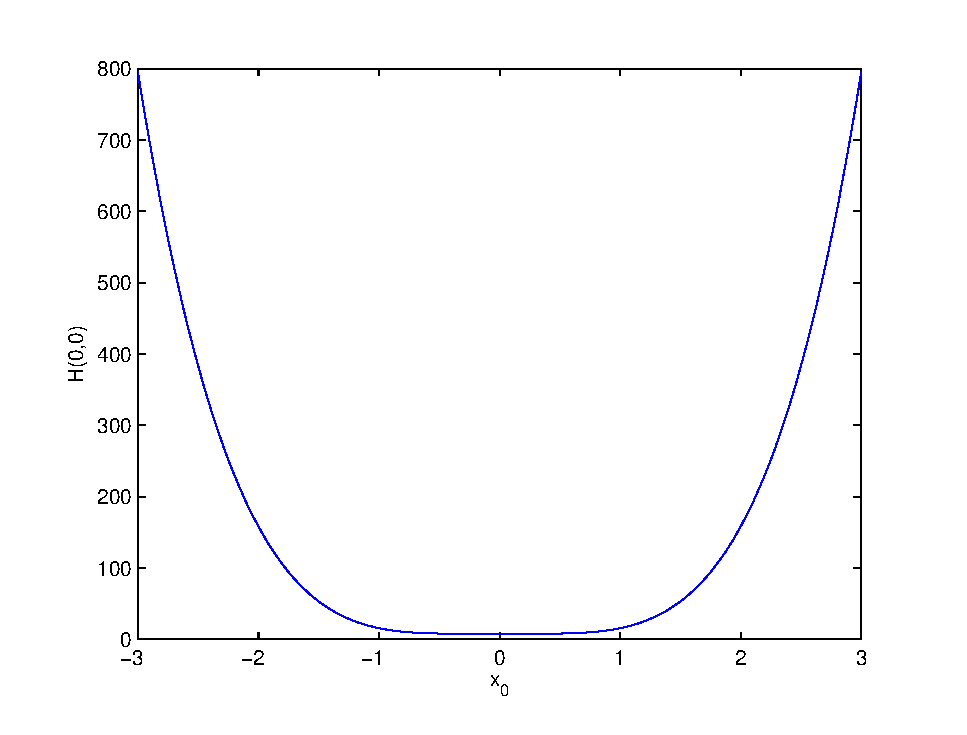
\includegraphics[scale=0.3]{figures/shcb_h00.eps}
	\label{fig:shcb_h00_nozoom}
}
\subfigure[$-0.8 \leq x_0 \leq 0.8$]{
	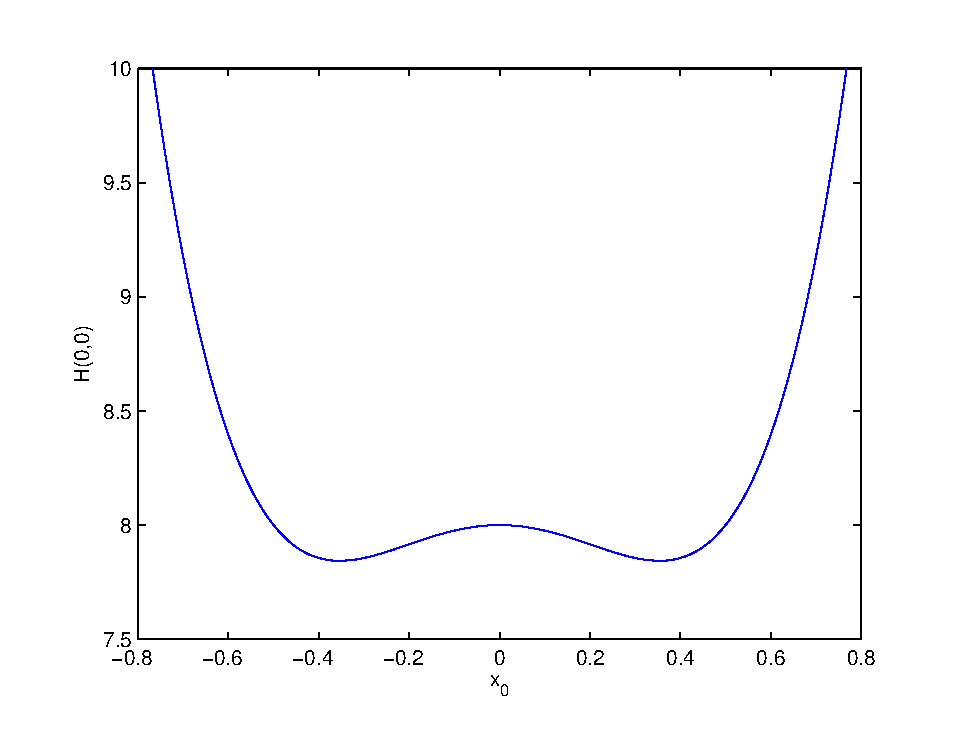
\includegraphics[scale=0.3]{figures/shcb_h00_zoom.eps}
	\label{fig:shcb_h00_zoom}
}
\caption{(0,0) element of Hessian defined in (\ref{eqn:shcb_hessian}).}
\label{fig:shcb_h00}
\end{figure}
The same goes for the (1,1) element, except that this is even easier since it is only a second degree polynomial, and it is convex (see fig. \ref{fig:shcb_h11}). Here, the minimum and and maximum must be located either in $x_1^L$, $x_1^U$, or the stationary point at $(0,-8)$.
\begin{figure}[H]
\centering
\includegraphics[scale=0.3]{figures/shcb_h11}
\caption{(1,1) element of Hessian defined in (\ref{eqn:shcb_hessian}) ($-2 \leq x_1 \leq 2$).}
\label{fig:shcb_h11}
\end{figure}
We create a new constraint class which we name \class{ConstraintSixHumpCamelWithRelaxation}, which starts out the same as the \class{ConstraintSixHumpCamel} class. That is, our starting point is the following header file:
\begin{lstlisting}
#ifndef CONSTRAINTSIXHUMPCAMELWITHRELAXATION_H
#define CONSTRAINTSIXHUMPCAMELWITHRELAXATION_H
#include "constraint.h"

class ConstraintSixHumpCamelWithRelaxation : public Constraint
{
public:
    ConstraintSixHumpCamelWithRelaxation();
    
    // Clone function - uses copy constructor
    virtual ConstraintSixHumpCamelWithRelaxation* clone() const {return new ConstraintSixHumpCamelWithRelaxation(*this);}

    virtual void evalF(DenseVector & x,DenseVector & y);

    virtual void evalGradF(DenseVector & x,DenseVector & dx);

    virtual void evalHessianF(DenseVector& x,DenseVector & ddx);

    virtual void structureGradF(std::vector< int >& iRow, std::vector< int >& jCol);

    virtual void structureHessianF(std::vector< int >& eqnr,std::vector< int >& iRow, std::vector< int >& jCol); 
};

#endif // CONSTRAINTSIXHUMPCAMELWITHRELAXATION_H
\end{lstlisting}
We now go through the steps required to modify this class to allow global optimization. These steps are:
\begin{itemize}
\item Add a pointer to a relaxed constraint as a private data member
\item Modify the constructor
\item Implement the copy constructor
\item Implement the \texttt{setDomainBounds()} function
\item Implement the \texttt{computeConvexRelaxation()} and \texttt{getConvexRelaxation()} functions
\item Create a new constraint class to represent the convex relaxation
\item Solve the optimization problem in a Branch-and-Bound framework
\end{itemize}

\paragraph{Add a pointer to a relaxed constraint as a private data member.} We add the following in the header file:
\begin{lstlisting}
private:
	ConstraintPtr relaxedConstraint;
\end{lstlisting}
This is a pointer to the relaxation of the constraint.  In the Branch-and-Bound framework, many instances of the constraint will be created, and each instance maintains its own relaxed constraint.

\paragraph{Modify the constructor.} We need to make some changes to the constructor:
\begin{itemize}
\item We have to set the constraint property \texttt{convexRelaxationAvailable} to \texttt{true}, to tell the Branch-and-Bound framework that this constraint has a convex relaxation available. The easiest way to accomplish this is to change the corresponding parameter of the \texttt{setConstraintProperties} function.
\item We have to create a convex relaxation of the constraint along with the constraint itself. To do this, we need to know the domain bounds. Therefore, we add two parameters to the constructor \texttt{lb} and \texttt{ub}, which are STL vectors of doubles. In the header file, the declaration becomes
\begin{lstlisting}
public:
	ConstraintSixHumpCamelWithRelaxation(std::vector< double > lb, std::vector< double > ub);
\end{lstlisting}
We use these parameters to update the \texttt{domainLowerBound} and \texttt{domainUpperBound} members, respectively. Now we can create some function \texttt{computeConvexRelaxation()} that uses these domain bounds to calculate the convex relaxation, and updates the \texttt{relaxedConstraint} member. We will define the function later, for now we just call it in the constructor.
\end{itemize}
The implementation in the .cpp file becomes:
\begin{lstlisting}
ConstraintSixHumpCamelWithRelaxation::ConstraintSixHumpCamelWithRelaxation(std::vector< double > lb, std::vector< double > ub):
	relaxedConstraint(nullptr)
{
	// Dimension of domain and codomain 
	dimensionDomainF = 3;
	dimensionCodomainF = 1;
	// Check consistency of domain bounds
	assert(lb.size() == ub.size());
	assert(lb.size() == dimensionDomainF);
	// Set domain bounds
	domainLowerBound = lb;
	domainUpperBound = ub;
	// Set the output bounds between -Inf and 0
	lowerBoundF.push_back(-IPOPT_UNBOUNDED);
	upperBoundF.push_back(0);
	// Gradient: true, Hessian: true, Linear: false, Convex: false, Convex relaxation: true
	setConstraintProperties(true, true, false, false, true);
	// Number of nonzero elements in the Jacobian and Hessian
	nnzGradient = 3;
	nnzHessian  = 3;
	// Compute convex relaxation
	computeConvexRelaxation();
	// Check settings for obvious mistakes
	checkConstraintSanity();
}
\end{lstlisting}

\paragraph{Implement the copy constructor.} The default copy constructor only copies the members of the object, not any objects they might be pointing to. In this case, the smart pointer \texttt{relaxedConstraint} will be copied, but the \class{ConstraintSixHumpCamelConvexRelaxation} object it points to will not. This is illustrated in fig. \ref{fig:nodeepcopy}. This behaviour will cause problems when one of the constraint objects makes changes to its relaxation, since these changes then will also apply to the copy of the constraint (which has made no such changes to its relaxation).
\begin{figure}[H]
\centering
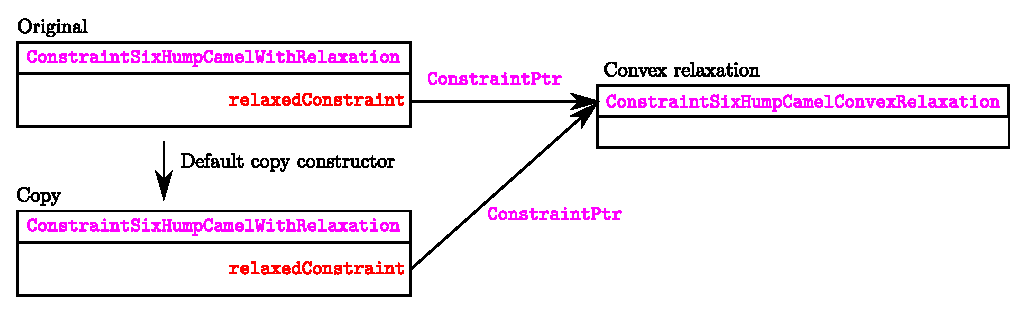
\includegraphics[scale=0.7]{figures/nodeepcopy.eps}
\caption{Default copy constructor behaviour.}
\label{fig:nodeepcopy}
\end{figure}
The solution is to implement a copy constructor that clones the relaxed constraint as well, so that the copy of the constraint gets its very own instance of the relaxed constraint. This is illustrated in fig. \ref{fig:deepcopy}.
\begin{figure}[H]
\centering
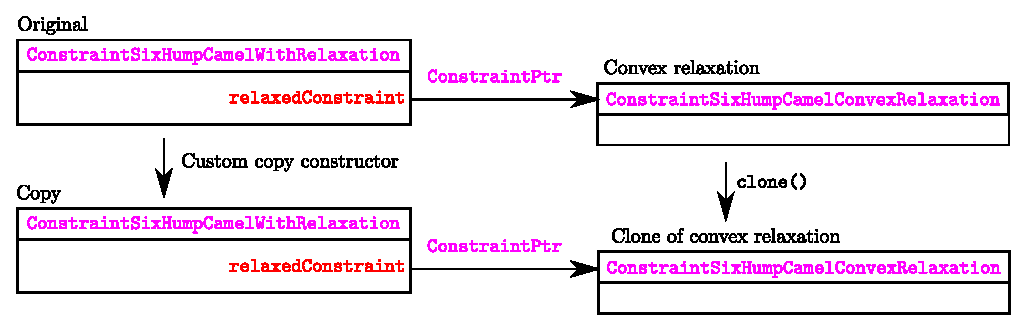
\includegraphics[scale=0.7]{figures/deepcopy.eps}
\caption{Desired copy constructor behaviour.}
\label{fig:deepcopy}
\end{figure}
To accomplish this, we add the declaration in the header file:
\begin{lstlisting}
public:							ConstraintSixHumpCamelWithRelaxation(ConstraintSixHumpCamelWithRelaxation const& copy);
\end{lstlisting}
and the implementation in the .cpp file:
\begin{lstlisting}
ConstraintSixHumpCamelWithRelaxation::ConstraintSixHumpCamelWithRelaxation(ConstraintSixHumpCamelWithRelaxation const& copy)
    : Constraint(copy)
{
	if (copy.relaxedConstraint == nullptr)
	{
		relaxedConstraint = nullptr;
	}
	else
	{
		relaxedConstraint = ConstraintPtr(copy.relaxedConstraint->clone());
	}
}
\end{lstlisting}
Note that we have to check whether the relaxation of the constraint we are trying to copy exists or not, before we call the \texttt{clone()} function to create a copy of the relaxation. Also, note that we also call the default copy constructor of the \class{Constraint} class (\texttt{: Constraint(copy)}) to copy all the basic constraint properties.

\paragraph{Implement the \texttt{setDomainBounds()} function.} When the domain bounds are changed, we must also calculate a new convex relaxation, since the relaxation changes when the bounds change. To do this, we overload the \texttt{setDomainBounds()} function of the \class{Constraint} class to include the calculation of a new relaxation:
\begin{lstlisting}
void ConstraintSixHumpCamelWithRelaxation::setDomainBounds(std::vector< double > lb, std::vector< double > ub)
{
	// Check parameters
	assert(lb.size() == dimensionDomainF);
	assert(ub.size() == dimensionDomainF);
	// Avoid unnecessary updates
	if (compareVec(lb,domainLowerBound) && compareVec(ub,domainUpperBound)) return;
	// Set domain bounds
	Constraint::setDomainBounds(lb, ub);
	// Recalculate the convex relaxation
	computeConvexRelaxation();
}
\end{lstlisting}

\paragraph{Implement the \texttt{computeConvexRelaxation()} and \texttt{getConvexRelaxation()} functions.} To implement these functions, we need equations (\ref{eqn:alpha}) and (\ref{eqn:mineigenval}). The function \texttt{computeConvexRelaxation()} is declared a private function:
\begin{lstlisting}
private:
	void computeConvexRelaxation();
\end{lstlisting}
Its implementation looks like this:
\begin{lstlisting}
void ConstraintSixHumpCamelWithRelaxation::computeConvexRelaxation()
{
	// Matrices to represent the interval Hessian
	DenseMatrix H_lo, H_hi;
	// Compute interval Hessian (depends on current domain bounds)
	intervalHessian(H_lo, H_hi);
	// Calculate lower bound on minimum eigenvalue
	double minEigenVal = minIntervalEigenValue(H_lo, H_hi);
	// Calculate required value for alpha
	double alpha = fmax(0, -0.5*minEigenVal);

	// Create new relaxed constraint based on alpha
	relaxedConstraint = ConstraintPtr(new ConstraintSixHumpCamelConvexRelaxation(domainLowerBound, domainUpperBound, alpha));
}
\end{lstlisting}
The first line:
\begin{lstlisting}
// Matrices to represent the interval Hessian
DenseMatrix H_lo, H_hi;
\end{lstlisting}
declares two matrices \texttt{H\_lo} and \texttt{H\_hi}, which represent the lower and upper bounds on the elements of the Hessian (\ref{eqn:shcb_hessian}). These bounds are calculated in the second line:
\begin{lstlisting}
// Compute interval Hessian (depends on current domain bounds)
intervalHessian(H_lo, H_hi);
\end{lstlisting}
The function \texttt{intervalHessian} has the declaration
\begin{lstlisting}
private:
	void intervalHessian(DenseMatrix& H_lo, DenseMatrix& H_hi);
\end{lstlisting}
and the implementation (refer to the comments to see exactly what the function does):
\begin{lstlisting}
void ConstraintSixHumpCamelWithRelaxation::intervalHessian(DenseMatrix &H_lo, DenseMatrix &H_hi)
{
	// The Hessian of the six hump camelback function has the following form:
	//
	//     | 8 - 25.2x0^2 + 10x0^4       1      0 |
	// H = |         1              48x1^2 - 8  0 |
	//     |         0                   0      0 |
	//
	// When the bounds on x0 and x1 are given, it is easy to
	// find bounds on the elements of the Hessian matrix.
	// The only non-constant elements are the (0,0) element
	// and the (1,1) element. The (0,0) element has three 
	// stationary points at x0 = 0, x0 = +/- 1.2249722
	// where the function value is 8 and -7.876, respectively.
	// The (1,1) element has one stationary point at x1 = 0,
	// where the function value is -8.

	// x0 and x1 must be bounded for us to be able to find an
	// interval Hessian.
	// Upper bound on x0
	assert(domainUpperBound.at(0) < IPOPT_UNBOUNDED);
	// Upper bound on x1   
	assert(domainUpperBound.at(1) < IPOPT_UNBOUNDED);  
	// Lower bound on x0 
	assert(domainLowerBound.at(0) > -IPOPT_UNBOUNDED);  
	// Lower bound on x1
	assert(domainLowerBound.at(1) > -IPOPT_UNBOUNDED);  

	// Max/min candidates
	std::vector< double > maxMinCandidates;

	// Find bounds on (0,0) element
	double statPoint1 = -1.2249722;  // Stationary points
	double statPoint2 = 0;
	double statPoint3 = 1.12249722;

	// Extreme points (at lower/upper bound)
	double y0L, y0U, x0L, x0U;
	x0L = domainLowerBound.at(0);
	x0U = domainUpperBound.at(0);
	y0L = 8 - 25.2 * pow(x0L, 2) + 10 * pow(x0L, 4);
	y0U = 8 - 25.2 * pow(x0U, 2) + 10 * pow(x0U, 4);
	maxMinCandidates.push_back(y0L);
	maxMinCandidates.push_back(y0U);

	// Stationary points are added to candidate points
	// if they are within the domain bounds
	if (valueWithinBounds(statPoint1, 0)) maxMinCandidates.push_back(-7.876);  // Value at x0 = -1.2249722
	if (valueWithinBounds(statPoint2, 0)) maxMinCandidates.push_back(0);       // Value at x0 = 0
	if (valueWithinBounds(statPoint3, 0)) maxMinCandidates.push_back(-7.876);  // Value at x0 = 1.2249722
	
	// Find the largest and smalles elements in the vector of
	// max/min candidates
	double maxElem00 = *std::max_element(maxMinCandidates.begin(), maxMinCandidates.end());
	double minElem00 = *std::min_element(maxMinCandidates.begin(), maxMinCandidates.end());

	maxMinCandidates.clear();

	// Find bounds on (1,1) element
	double y1L, y1U, x1L, x1U;
	x1L = domainLowerBound.at(1);
	x1U = domainUpperBound.at(1);
	y1L = 48 * pow(x1L, 2) - 8;
	y1U = 48 * pow(x1U, 2) - 8;
	maxMinCandidates.push_back(y1L);
	maxMinCandidates.push_back(y1U);
	if (valueWithinBounds(0, 1)) maxMinCandidates.push_back(-8);  // Value at x1 = 0
	
	// Find the largest and smalles elements in the vector of
	// max/min candidates
	double maxElem11 = *std::max_element(maxMinCandidates.begin(), maxMinCandidates.end());
	double minElem11 = *std::min_element(maxMinCandidates.begin(), maxMinCandidates.end());

	// Fill out upper/lower bounds
	H_lo.setZero(3, 3);
	H_lo(0,0) = minElem00;
	H_lo(0,1) = 1;
	H_lo(1,0) = 1;
	H_lo(1,1) = minElem11;
	H_hi.setZero(3, 3);
	H_hi(0,0) = maxElem00;
	H_hi(0,1) = 1;
	H_hi(1,0) = 1;
	H_hi(1,1) = maxElem11;
}
\end{lstlisting}
This function uses the function \texttt{valueWithinBounds(double value, int varNo)}, which only checks whether \texttt{value} lies within the domain bounds of variable number \texttt{varNo}. The declaration is
\begin{lstlisting}
private:
	bool valueWithinBounds(double value, int varNo);
\end{lstlisting}
and the implementation is:
\begin{lstlisting}
bool ConstraintSixHumpCamelWithRelaxation::valueWithinBounds(double value, int varNo)
{
	// Check that varNo is a valid variable index
	assert(varNo < dimensionDomainF);
	// Check if value is within bounds, return true/false
	if (domainLowerBound.at(varNo) <= value && domainUpperBound.at(varNo) >= value)
	{
		return true;
	}
	else
	{
		return false;
	}
}
\end{lstlisting}
Now that we have calculated bounds on each element in the Hessian, we can calculate a lower bound on the minimum eigenvalue of the Hessian. This is done in the third line:
\begin{lstlisting}
// Calculate lower bound on minimum eigenvalue
double minEigenVal = minIntervalEigenValue(H_lo, H_hi);
\end{lstlisting}
The function \texttt{minIntervalEigenValue} is nothing else than an application of (\ref{eqn:mineigenval}). The declaration is
\begin{lstlisting}
private:
	double minIntervalEigenValue(DenseMatrix& H_lo, DenseMatrix& H_hi);
\end{lstlisting}
and the implementation is
\begin{lstlisting}
double ConstraintSixHumpCamelWithRelaxation::minIntervalEigenValue(DenseMatrix &H_lo, DenseMatrix &H_hi)
{
    // Uses Thm. 3.2 in Adjiman et. al (1998) to find a lower
    // bound on the minimum eigenvalue of the interval matrix
    // given by H_lo and H_hi.

    // Check that both matrices are square and that they are
    // the same size
    assert(H_lo.rows() == H_lo.cols());
    assert(H_hi.rows() == H_hi.cols());
    assert(H_lo.rows() == H_hi.rows());
    assert(H_lo.cols() == H_hi.cols());

    int dim = H_lo.rows();

    double minEigenVal = IPOPT_UNBOUNDED;
    for (int i = 0; i < dim; i++)
    {
        double minCandidate = H_lo(i,i);
        for (int j = 0; j < dim; j++)
        {
            if (i != j)
            {
                minCandidate -= fmax( fabs(H_lo(i,j)) , fabs(H_hi(i,j)));
            }
        }
        if (minCandidate < minEigenVal)
        {
            minEigenVal = minCandidate;
        }
    }
    return minEigenVal;
}
\end{lstlisting}
We use the obtained bound to calculate the required value of $\alpha$ with (\ref{eqn:alpha}) in line four:
\begin{lstlisting}
// Calculate required value for alpha
double alpha = fmax(0, -0.5*minEigenVal);
\end{lstlisting}
and pass this value to the constructor of the relaxed constraint class in the fifth and final line:
\begin{lstlisting}
// Create new relaxed constraint based on alpha
	relaxedConstraint = ConstraintPtr(new ConstraintSixHumpCamelConvexRelaxation(domainLowerBound, domainUpperBound, alpha));
\end{lstlisting}
The function \texttt{getConvexRelaxation()} simply clones the relaxed constraint and returns a pointer to the clone. It has the declaration
\begin{lstlisting}
public:
	virtual Constraint* getConvexRelaxation() const;
\end{lstlisting}
and the implementation
\begin{lstlisting}
Constraint* ConstraintSixHumpCamelWithRelaxation::getConvexRelaxation() const
{
	assert(relaxedConstraint != nullptr);
	return relaxedConstraint->clone();
}
\end{lstlisting}

\paragraph{Create a new constraint class to represent the convex relaxation.} We need to create a new class to represent the convex relaxations. We will call it \class{ConstraintSixHumpCamelConvexRelaxation}. The implementation of this class will be very similar to the implementation of the \class{ConstraintSixHumpCamel} class from section \ref{sec:shcb_custom}, with a few differences:
\begin{itemize}
\item The function, Jacobian and Hessian evaluations are obviously slightly different.
\item The constructor takes the domain bounds as parameters as these are used in the function evaluations.
\item It contains the private data member \texttt{alpha}, which is also used in the function evaluations.
\item The constraint properties \texttt{constraintConvex} and \texttt{convexRelaxationAvailable} are set to \texttt{true}.
\end{itemize}
Let the convex relaxation of $c_1(x)$ be denoted $\underline{c}_1(x)$. Then we have
\begin{align*}
\underline{c}_1(x) &= f_{\mathrm{SH}}(x_0,x_1) + \alpha (x_0^L - x_0)(x_0^U - x_0) + \alpha (x_1^L - x_1)(x_1^U - x_1) - x_2 \\
&= \left( 4 - 2.1x_0^2 + \frac{x_0^4}{3} \right)x_0^2 + x_0x_1 + (-4 + 4x_1^2) x_1^2 \\
&\ \ \ + \alpha (x_0^L - x_0)(x_0^U - x_0) + \alpha (x_1^L - x_1)(x_1^U - x_1) - x_2
\end{align*}
The gradient $\nabla \underline{c}_1(x)$ is
\begin{align*}
\nabla \underline{c}_1(x) &= \begin{bmatrix} 8x_0 - 8.4 x_0^3 + 2x_0^5 + x_1 + 2\alpha x_0 - \alpha(x_0^L + x_0^U) \\ x_0 - 8x_1 + 16x_1^3 + 2\alpha x_1 - \alpha (x_1^L + x_1^U) \\ -1 \end{bmatrix}^\top.
\end{align*}
The Hessian $\nabla^2 \underline{c}_1(x)$ is
\begin{align*}
\nabla^2 \underline{c}_1(x) &= \begin{bmatrix} 8 - 25.2x_0^2 + 10x_0^4 + 2\alpha & 1 & 0 \\ 1 & 48x_1^2 - 8 + 2\alpha & 0 \\ 0 & 0 & 0 \end{bmatrix}.
\end{align*}
This gives us the header file
\begin{lstlisting}
#ifndef CONSTRAINTSIXHUMPCAMELCONVEXRELAXATION_H
#define CONSTRAINTSIXHUMPCAMELCONVEXRELAXATION_H

#include "constraint.h"

class ConstraintSixHumpCamelConvexRelaxation : public Constraint
{
public:
	ConstraintSixHumpCamelConvexRelaxation(std::vector< double > lb, std::vector< double > ub, double alpha);

	// Clone function - uses copy constructor
	virtual ConstraintSixHumpCamelConvexRelaxation* clone() const {return new ConstraintSixHumpCamelConvexRelaxation(*this);}

	virtual void evalF(DenseVector & x,DenseVector & y);

	virtual void evalGradF(DenseVector & x,DenseVector & dx);

	virtual void evalHessianF(DenseVector& x,DenseVector & ddx);

	virtual void structureGradF(std::vector< int >& iRow, std::vector< int >& jCol);

	virtual void structureHessianF(std::vector< int >& eqnr,std::vector< int >& iRow, std::vector< int >& jCol);

private:
	double alpha;
};

#endif // CONSTRAINTSIXHUMPCAMELCONVEXRELAXATION_H
\end{lstlisting}
and the .cpp file
\begin{lstlisting}
#include "constraintsixhumpcamelconvexrelaxation.h"

ConstraintSixHumpCamelConvexRelaxation::ConstraintSixHumpCamelConvexRelaxation(std::vector< double > lb, std::vector< double > ub, double alpha)
{
	dimensionDomainF = 3;
	dimensionCodomainF = 1;

	gradientCalculatedF = true;
	hessianCalculatedF = true;

	assert(lb.size() == ub.size());
	assert(lb.size() == dimensionDomainF);

	domainLowerBound = lb;
	domainUpperBound = ub;

	lowerBoundF.push_back(-IPOPT_UNBOUNDED);
	upperBoundF.push_back(0);

	this->alpha = alpha;

	// Gradient: true, Hessian: true, Linear: false, Convex: true, Convex relaxation: true
	setConstraintProperties(true, true, false, true, true);

	nnzGradient = 3;
	nnzHessian  = 3;

	checkConstraintSanity();
}

void ConstraintSixHumpCamelConvexRelaxation::evalF(DenseVector & x,DenseVector & y)
{
    double x0L = domainLowerBound.at(0);
	double x0U = domainUpperBound.at(0);
	double x1L = domainLowerBound.at(1);
	double x1U = domainUpperBound.at(1);

	double t1 = (4.0-2.1*pow(x(0),2)+pow(x(0),4)/3.0)*pow(x(0),2);
	double t2 = x(0)*x(1);
	double t3 = (-4+4*pow(x(1),2))*pow(x(1),2);
	double t4 = alpha*(x0L*x0U-x(0)*(x0L+x0U)+pow(x(0),2));	
    double t5 = alpha*(x1L*x1U-x(1)*(x1L+x1U)+pow(x(1),2));

	y(0) = t1+t2+t3+t4+t5-x(2);
}

void ConstraintSixHumpCamelConvexRelaxation::evalGradF(DenseVector & x,DenseVector & dx)
{
	double x0L = domainLowerBound.at(0);
	double x0U = domainUpperBound.at(0);
	double x1L = domainLowerBound.at(1);
	double x1U = domainUpperBound.at(1);
	dx(0) = 8*x(0)-8.4*pow(x(0),3)+2*pow(x(0),5)+x(1)+2*alpha*x(0)-alpha*(x0L+x0U);
	dx(1) = x(0)-8*x(1)+16*pow(x(1),3)+2*alpha*x(1)-alpha*(x1L+x1U);
	dx(2) = -1;
}

void ConstraintSixHumpCamelConvexRelaxation::evalHessianF(DenseVector& x,DenseVector & ddx)
{
	ddx(0) = 8-25.2*pow(x(0),2)+10*pow(x(0),4)+2*alpha;
	ddx(1) = 1;
	ddx(2) = -8+48*pow(x(1),2)+2*alpha;
}

void ConstraintSixHumpCamelConvexRelaxation::structureGradF(std::vector< int > &iRow, std::vector< int > &jCol)
{
	iRow.push_back(0); jCol.push_back(0);
	iRow.push_back(0); jCol.push_back(1);
	iRow.push_back(0); jCol.push_back(2);
}

void ConstraintSixHumpCamelConvexRelaxation::structureHessianF(std::vector< int > &eqnr, std::vector< int > &iRow, std::vector< int > &jCol)
{
	eqnr.push_back(0);	iRow.push_back(0);	jCol.push_back(0);
	eqnr.push_back(0);	iRow.push_back(0);	jCol.push_back(1);
	eqnr.push_back(0);	iRow.push_back(1);	jCol.push_back(1);
}
\end{lstlisting}

\paragraph{Solve the optimization problem in a Branch-and-Bound framework.} We will now use the \class{ConstraintSixHumpCamelWithRelaxation} class we created in the paragraphs above to solve the Six-Hump Camelback problem globally. First, we create an instance of the constraint and add it to the constraint composite as we have done earlier:
\begin{lstlisting}
ConstraintPtr cSixHump(new ConstraintSixHumpCamelWithRelaxation(lb, ub));
constraints->add(cSixHump, variableMapping);
\end{lstlisting}
In addition to the constraints and objective function, the Branch-and-Bound framework needs to know the variable types (continuous/integer) and which variables should be branced on. In our case, all variables are continuous and $x_0$ and $x_1$ are the branching variables. We create two STL integer vectors and insert the correct variable indices:
\begin{lstlisting}
std::vector< int > variable_types;
variable_types.push_back(CONTINUOUS); // x0
variable_types.push_back(CONTINUOUS); // x1
variable_types.push_back(CONTINUOUS); // x2

std::vector< int > branching_variables;
branching_variables.push_back(0);
branching_variables.push_back(1);
\end{lstlisting}
Now we can create a \class{BranchAndBound} object, which takes the objective, constraints, starting point, variable types and branching variables as parameters, and call its \texttt{optimize()} function to run the Branch-and-Bound algorithm:
\begin{lstlisting}
BranchAndBound bnb(objective, constraints, z0, variable_types, branching_variables);
bnb.optimize();    
\end{lstlisting}
The optimal point and objective function value are available through the \texttt{getOptimalSolution()} and \texttt{getObjectiveValue()} functions, respectively:
\begin{lstlisting}
zopt_found = bnb.getOptimalSolution();
fopt_found = bnb.getObjectiveValue();
\end{lstlisting}
The Branch-and-Bound algorithm finds the global optimum, but achieving epsilon-convergence takes a long time due to the poor quality of the convex relaxations. For instance, with the starting point $z_0 = (0, 0, 0)$, it takes 2671 iterations to achieve epsilon-convergence (see fig. \ref{fig:shcb_progress1}), and with the starting point $z_0 = (1,0,0)$ it takes 4031 iterations (fig. \ref{fig:shcb_progress2}). However, the global optimal point is found  within a few iterations; it is the shrinking of the optimality gap (our certificate of a global solution) that takes a long time.
\begin{figure}[H]
\centering
\subfigure[$z_0 = (0,0,0)$]{
	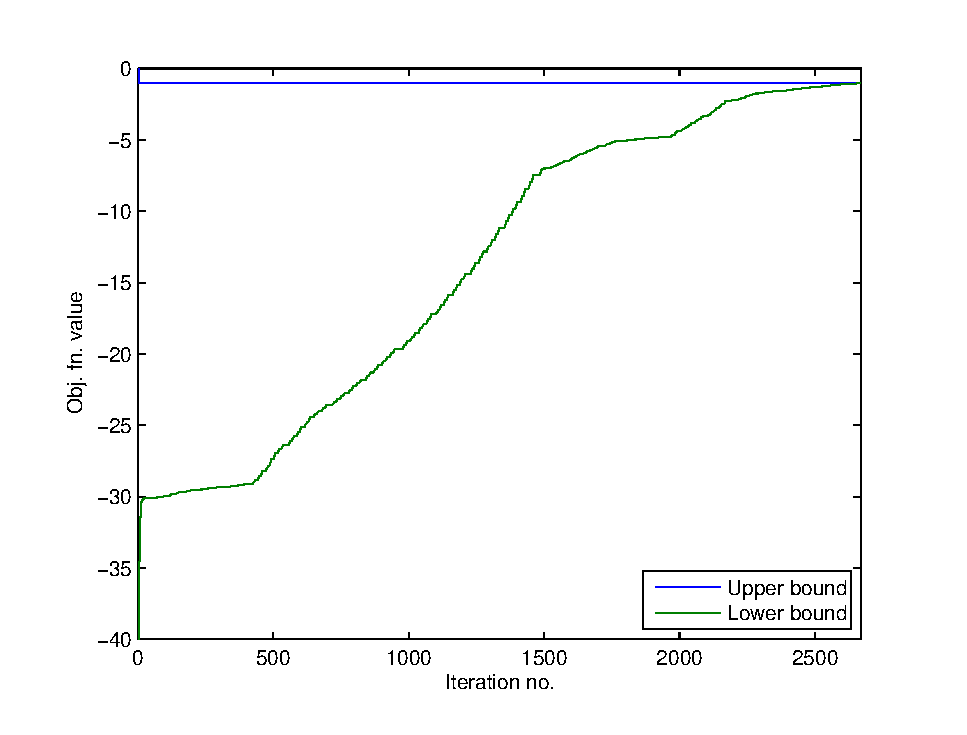
\includegraphics[width=0.45\textwidth]{figures/shcb_progress1.eps}
	\label{fig:shcb_progress1}
}
\subfigure[$z_0 = (1,0,0)$]{
	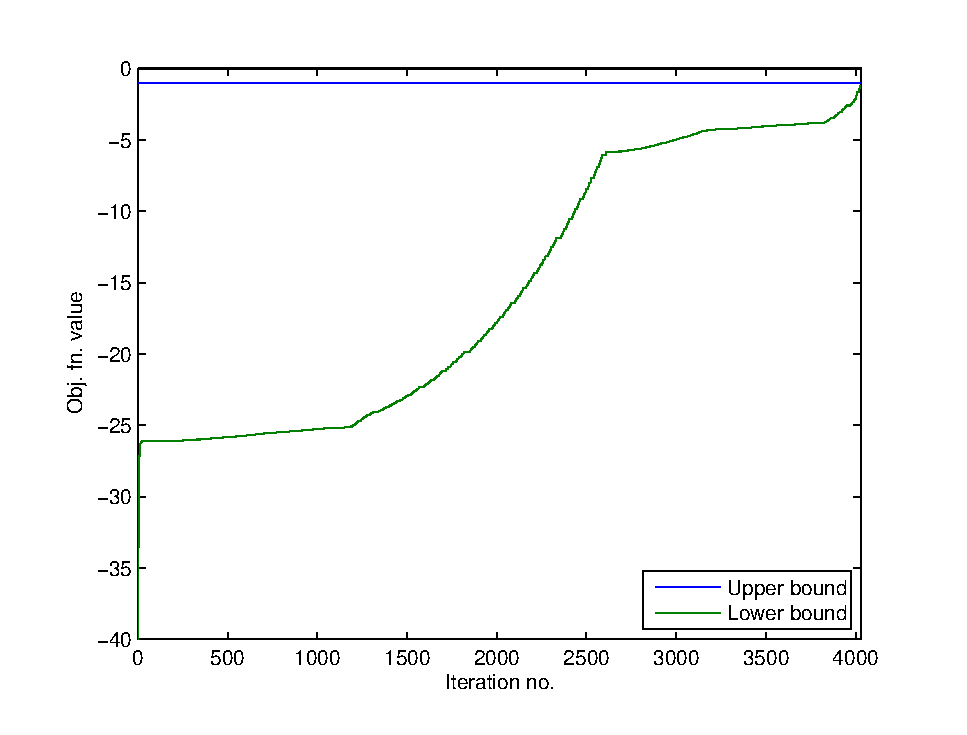
\includegraphics[width=0.45\textwidth]{figures/shcb_progress2.eps}
	\label{fig:shcb_progress2}
}
\caption{Branch-and-Bound algorithm progress with the $\alpha$BB approach.}
\label{fig:shcb_progress}
\end{figure}

\subsubsection{Global optimization using a B-spline approximation}
\label{sec:shcb_bspline}
The methods desribed in the paragraphs above are time consuming and error-prone. An easier approach is to use a B-spline approximation of the Six-Hump Camelback function to solve the problem globally. As mentioned in section \ref{sec:bspline}, an attractive property of the B-spline is that the control points used to describe the B-spline can be used to construct a convex relaxation of the B-spline. This property has been exploited in the \class{ConstraintBspline} class, meaning that we can solve problems defined with B-splines globally. To solve the Six-Hump Camelback problem with this approach, we have to complete the following steps:
\begin{itemize}
\item
Create an \class{InterpolationTable} object and fill it with samples
\item
Create a B-spline constraint using the interpolation table
\item
Add the constraint to the constraint composite
\item
Solve the optimization problem in a Branch-and-Bound framework
\end{itemize}

\paragraph{Create an \class{InterpolationTable} object and fill it with samples.} The B-spline constraint constructor takes three parameters; an interpolation table filled with samples, the desired degree of the polynomial pieces from which the B-spline is constructed, and a boolean value to indicate equality or inequality. First, we create a function to evaluate the Six-Hump Camelback function itself:
\begin{lstlisting}
DenseVector sixHumpCamelFunction(DenseVector x)
{
    assert(x.rows() == 2);
    DenseVector y; y.setZero(1);
    y(0) = (4 - 2.1*x(0)*x(0) + (1/3.)*x(0)*x(0)*x(0)*x(0))*x(0)*x(0) + x(0)*x(1) + (-4 + 4*x(1)*x(1))*x(1)*x(1);
    return y;
}
\end{lstlisting}
Now, we use this function to evaluate the Six-Hump Camelback function in a grid (see section \ref{sec:interpolationtable} for details on the \class{InterpolationTable} class).
\begin{lstlisting}
InterpolationTable* data = new InterpolationTable(2, 1, false);

double dx = 0.05;
for (double x1 = lb.at(0); x1 <= ub.at(0); x1+=dx)
{
	for (double x2 = lb.at(1); x2 <= ub.at(1); x2+=dx)
	{
		std::vector< double > x;
		x.push_back(x1);
		x.push_back(x2);

		DenseVector xd; xd.setZero(2);
		xd(0) = x1;
		xd(1) = x2;
		DenseVector yd = sixHumpCamelFunction(xd);

		data->addSample(x,yd(0));
	}
}
\end{lstlisting}

\paragraph{Create a B-spline constraint using the interpolation table.} We select a polynomial degree of 3, since this gives us a B-spline which is twice continuously differentiable. We set the third parameter to \texttt{true} to indicate that we want an equality constraint.
\begin{lstlisting}
ConstraintPtr cbspline(new ConstraintBspline(*data, 3, true));
\end{lstlisting}

\paragraph{Add the constraint to the constraint composite.} As before,
\begin{lstlisting}
constraints->add(cbspline, variableMapping);
\end{lstlisting}

\paragraph{Solve the optimization problem in a Branch-and-Bound framework.} This is done in the same way as described for the $\alpha$BB approach; we create two STL vectors with variable types and brancing variables, and pass these to a \class{BranchAndBound} object along with the objective, constraints and starting point:
\begin{lstlisting}
std::vector< int > variable_types;
variable_types.push_back(CONTINUOUS); // x0
variable_types.push_back(CONTINUOUS); // x1
variable_types.push_back(CONTINUOUS); // x2
std::vector< int > branching_variables;
branching_variables.push_back(0);
branching_variables.push_back(1);

BranchAndBound bnb(objective, constraints, z0, variable_types, branching_variables);
bnb.optimize();    

zopt_found = bnb.getOptimalSolution();
fopt_found = bnb.getObjectiveValue();
\end{lstlisting}
This time, the problem is solved in only 49 iterations. The large improvement in performance is due to the improved quality of the convex relaxations. The progress of the algorithm is shown in fig. \ref{fig:shcb_progress3}. Note that the initial lower bound is very close to the upper bound (< 0.01 as opposed to > 25-30 for the $\alpha$BB approach).
\begin{figure}[H]
\centering
\includegraphics[width=\textwidth]{figures/shcb_progress3.eps}
\caption{Branch-and-Bound algorithm progress with the B-spline approach.}
\label{fig:shcb_progress3}
\end{figure}
Since we are using an approximation, the optimal solution will have an error. However, this error becomes smaller when we increase the number of samples.
